% Created by tikzDevice version 0.7.0 on 2014-07-29 12:04:21
% !TEX encoding = UTF-8 Unicode
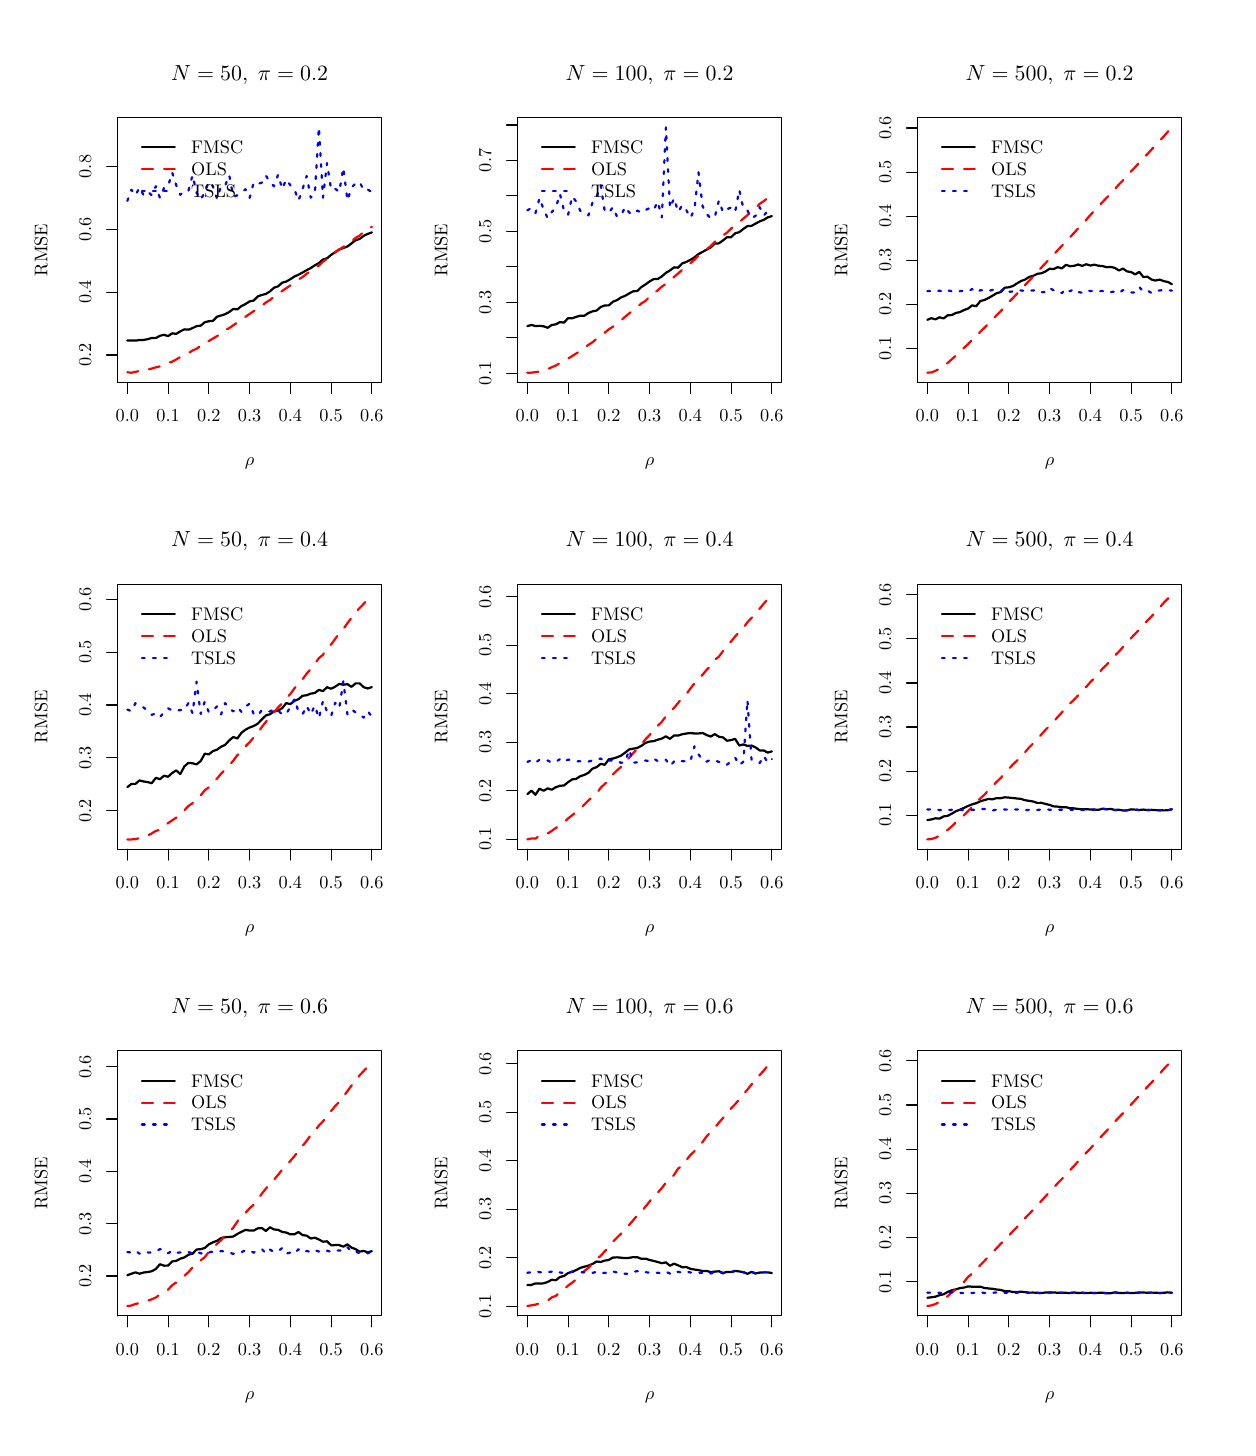
\begin{tikzpicture}[x=1pt,y=1pt]
\definecolor[named]{fillColor}{rgb}{1.00,1.00,1.00}
\path[use as bounding box,fill=fillColor,fill opacity=0.00] (0,0) rectangle (433.62,505.89);
\begin{scope}
\path[clip] ( 32.47,377.65) rectangle (127.91,473.42);
\definecolor[named]{drawColor}{rgb}{0.00,0.00,0.00}

\path[draw=drawColor,line width= 0.8pt,line join=round,line cap=round] ( 36.01,392.85) --
	( 37.48,392.85) --
	( 38.95,392.82) --
	( 40.42,392.99) --
	( 41.90,393.05) --
	( 43.37,393.32) --
	( 44.84,393.76) --
	( 46.32,393.73) --
	( 47.79,394.55) --
	( 49.26,394.91) --
	( 50.73,394.44) --
	( 52.21,395.44) --
	( 53.68,395.23) --
	( 55.15,396.16) --
	( 56.63,396.88) --
	( 58.10,396.76) --
	( 59.57,397.32) --
	( 61.04,398.05) --
	( 62.52,398.20) --
	( 63.99,399.44) --
	( 65.46,399.81) --
	( 66.93,399.94) --
	( 68.41,401.44) --
	( 69.88,401.88) --
	( 71.35,402.35) --
	( 72.83,403.14) --
	( 74.30,404.25) --
	( 75.77,404.09) --
	( 77.24,405.29) --
	( 78.72,406.02) --
	( 80.19,406.97) --
	( 81.66,407.27) --
	( 83.14,408.76) --
	( 84.61,409.31) --
	( 86.08,409.66) --
	( 87.55,410.59) --
	( 89.03,411.92) --
	( 90.50,412.42) --
	( 91.97,413.74) --
	( 93.44,414.14) --
	( 94.92,415.00) --
	( 96.39,415.97) --
	( 97.86,416.61) --
	( 99.34,417.42) --
	(100.81,418.25) --
	(102.28,419.03) --
	(103.75,420.01) --
	(105.23,420.82) --
	(106.70,422.09) --
	(108.17,422.54) --
	(109.65,423.80) --
	(111.12,424.77) --
	(112.59,425.70) --
	(114.06,426.28) --
	(115.54,426.81) --
	(117.01,427.93) --
	(118.48,429.07) --
	(119.95,429.54) --
	(121.43,430.66) --
	(122.90,431.38) --
	(124.37,431.90);
\end{scope}
\begin{scope}
\path[clip] (  0.00,  0.00) rectangle (433.62,505.89);
\definecolor[named]{drawColor}{rgb}{0.00,0.00,0.00}

\path[draw=drawColor,line width= 0.4pt,line join=round,line cap=round] ( 36.01,377.65) -- (124.37,377.65);

\path[draw=drawColor,line width= 0.4pt,line join=round,line cap=round] ( 36.01,377.65) -- ( 36.01,373.69);

\path[draw=drawColor,line width= 0.4pt,line join=round,line cap=round] ( 50.73,377.65) -- ( 50.73,373.69);

\path[draw=drawColor,line width= 0.4pt,line join=round,line cap=round] ( 65.46,377.65) -- ( 65.46,373.69);

\path[draw=drawColor,line width= 0.4pt,line join=round,line cap=round] ( 80.19,377.65) -- ( 80.19,373.69);

\path[draw=drawColor,line width= 0.4pt,line join=round,line cap=round] ( 94.92,377.65) -- ( 94.92,373.69);

\path[draw=drawColor,line width= 0.4pt,line join=round,line cap=round] (109.65,377.65) -- (109.65,373.69);

\path[draw=drawColor,line width= 0.4pt,line join=round,line cap=round] (124.37,377.65) -- (124.37,373.69);

\node[text=drawColor,anchor=base,inner sep=0pt, outer sep=0pt, scale=  0.66] at ( 36.01,363.40) {0.0};

\node[text=drawColor,anchor=base,inner sep=0pt, outer sep=0pt, scale=  0.66] at ( 50.73,363.40) {0.1};

\node[text=drawColor,anchor=base,inner sep=0pt, outer sep=0pt, scale=  0.66] at ( 65.46,363.40) {0.2};

\node[text=drawColor,anchor=base,inner sep=0pt, outer sep=0pt, scale=  0.66] at ( 80.19,363.40) {0.3};

\node[text=drawColor,anchor=base,inner sep=0pt, outer sep=0pt, scale=  0.66] at ( 94.92,363.40) {0.4};

\node[text=drawColor,anchor=base,inner sep=0pt, outer sep=0pt, scale=  0.66] at (109.65,363.40) {0.5};

\node[text=drawColor,anchor=base,inner sep=0pt, outer sep=0pt, scale=  0.66] at (124.37,363.40) {0.6};

\path[draw=drawColor,line width= 0.4pt,line join=round,line cap=round] ( 32.47,387.59) -- ( 32.47,455.73);

\path[draw=drawColor,line width= 0.4pt,line join=round,line cap=round] ( 32.47,387.59) -- ( 28.51,387.59);

\path[draw=drawColor,line width= 0.4pt,line join=round,line cap=round] ( 32.47,410.30) -- ( 28.51,410.30);

\path[draw=drawColor,line width= 0.4pt,line join=round,line cap=round] ( 32.47,433.02) -- ( 28.51,433.02);

\path[draw=drawColor,line width= 0.4pt,line join=round,line cap=round] ( 32.47,455.73) -- ( 28.51,455.73);

\node[text=drawColor,rotate= 90.00,anchor=base,inner sep=0pt, outer sep=0pt, scale=  0.66] at ( 22.97,387.59) {0.2};

\node[text=drawColor,rotate= 90.00,anchor=base,inner sep=0pt, outer sep=0pt, scale=  0.66] at ( 22.97,410.30) {0.4};

\node[text=drawColor,rotate= 90.00,anchor=base,inner sep=0pt, outer sep=0pt, scale=  0.66] at ( 22.97,433.02) {0.6};

\node[text=drawColor,rotate= 90.00,anchor=base,inner sep=0pt, outer sep=0pt, scale=  0.66] at ( 22.97,455.73) {0.8};

\path[draw=drawColor,line width= 0.4pt,line join=round,line cap=round] ( 32.47,377.65) --
	(127.91,377.65) --
	(127.91,473.42) --
	( 32.47,473.42) --
	( 32.47,377.65);
\end{scope}
\begin{scope}
\path[clip] (  0.00,337.26) rectangle (144.54,505.89);
\definecolor[named]{drawColor}{rgb}{0.00,0.00,0.00}

\node[text=drawColor,anchor=base,inner sep=0pt, outer sep=0pt, scale=  0.79] at ( 80.19,486.92) {\bfseries $N=50, \;\pi=0.2$};

\node[text=drawColor,anchor=base,inner sep=0pt, outer sep=0pt, scale=  0.66] at ( 80.19,347.56) {$\rho$};

\node[text=drawColor,rotate= 90.00,anchor=base,inner sep=0pt, outer sep=0pt, scale=  0.66] at (  7.13,425.53) {RMSE};
\end{scope}
\begin{scope}
\path[clip] ( 32.47,377.65) rectangle (127.91,473.42);
\definecolor[named]{drawColor}{rgb}{1.00,0.00,0.00}

\path[draw=drawColor,line width= 0.8pt,dash pattern=on 4pt off 4pt ,line join=round,line cap=round] ( 36.01,381.36) --
	( 37.48,381.20) --
	( 38.95,381.49) --
	( 40.42,381.86) --
	( 41.90,381.80) --
	( 43.37,382.32) --
	( 44.84,382.70) --
	( 46.32,383.15) --
	( 47.79,383.49) --
	( 49.26,384.27) --
	( 50.73,384.73) --
	( 52.21,385.20) --
	( 53.68,385.99) --
	( 55.15,386.88) --
	( 56.63,387.76) --
	( 58.10,388.30) --
	( 59.57,389.22) --
	( 61.04,389.85) --
	( 62.52,390.94) --
	( 63.99,392.08) --
	( 65.46,392.66) --
	( 66.93,393.54) --
	( 68.41,394.43) --
	( 69.88,395.21) --
	( 71.35,396.60) --
	( 72.83,397.31) --
	( 74.30,398.35) --
	( 75.77,399.35) --
	( 77.24,400.35) --
	( 78.72,401.43) --
	( 80.19,402.45) --
	( 81.66,403.45) --
	( 83.14,404.48) --
	( 84.61,405.41) --
	( 86.08,406.58) --
	( 87.55,407.49) --
	( 89.03,408.69) --
	( 90.50,409.35) --
	( 91.97,410.77) --
	( 93.44,411.75) --
	( 94.92,412.75) --
	( 96.39,414.06) --
	( 97.86,414.89) --
	( 99.34,415.77) --
	(100.81,416.98) --
	(102.28,417.93) --
	(103.75,419.08) --
	(105.23,419.91) --
	(106.70,421.31) --
	(108.17,422.34) --
	(109.65,423.54) --
	(111.12,424.75) --
	(112.59,425.76) --
	(114.06,426.67) --
	(115.54,427.66) --
	(117.01,428.70) --
	(118.48,429.92) --
	(119.95,430.74) --
	(121.43,432.08) --
	(122.90,433.23) --
	(124.37,433.92);
\definecolor[named]{drawColor}{rgb}{0.00,0.00,1.00}

\path[draw=drawColor,line width= 0.8pt,dash pattern=on 1pt off 3pt ,line join=round,line cap=round] ( 36.01,443.28) --
	( 37.48,447.36) --
	( 38.95,445.30) --
	( 40.42,448.16) --
	( 41.90,445.34) --
	( 43.37,446.58) --
	( 44.84,445.36) --
	( 46.32,448.60) --
	( 47.79,444.35) --
	( 49.26,447.89) --
	( 50.73,448.59) --
	( 52.21,453.56) --
	( 53.68,448.94) --
	( 55.15,445.48) --
	( 56.63,446.88) --
	( 58.10,446.98) --
	( 59.57,452.57) --
	( 61.04,446.27) --
	( 62.52,443.76) --
	( 63.99,446.35) --
	( 65.46,450.26) --
	( 66.93,448.68) --
	( 68.41,444.07) --
	( 69.88,448.63) --
	( 71.35,448.80) --
	( 72.83,452.57) --
	( 74.30,444.85) --
	( 75.77,445.31) --
	( 77.24,446.26) --
	( 78.72,447.50) --
	( 80.19,444.39) --
	( 81.66,449.87) --
	( 83.14,449.37) --
	( 84.61,449.91) --
	( 86.08,452.43) --
	( 87.55,450.07) --
	( 89.03,448.57) --
	( 90.50,452.79) --
	( 91.97,447.62) --
	( 93.44,451.06) --
	( 94.92,448.97) --
	( 96.39,447.49) --
	( 97.86,443.41) --
	( 99.34,447.60) --
	(100.81,452.30) --
	(102.28,444.47) --
	(103.75,445.83) --
	(105.23,469.87) --
	(106.70,444.43) --
	(108.17,456.95) --
	(109.65,447.37) --
	(111.12,447.67) --
	(112.59,446.52) --
	(114.06,455.25) --
	(115.54,443.48) --
	(117.01,448.03) --
	(118.48,449.65) --
	(119.95,450.13) --
	(121.43,447.14) --
	(122.90,447.40) --
	(124.37,446.42);
\definecolor[named]{drawColor}{rgb}{0.00,0.00,0.00}

\path[draw=drawColor,line width= 0.8pt,line join=round,line cap=round] ( 41.28,462.63) -- ( 53.16,462.63);
\definecolor[named]{drawColor}{rgb}{1.00,0.00,0.00}

\path[draw=drawColor,line width= 0.8pt,dash pattern=on 4pt off 4pt ,line join=round,line cap=round] ( 41.28,454.71) -- ( 53.16,454.71);
\definecolor[named]{drawColor}{rgb}{0.00,0.00,1.00}

\path[draw=drawColor,line width= 0.8pt,dash pattern=on 1pt off 3pt ,line join=round,line cap=round] ( 41.28,446.79) -- ( 53.16,446.79);
\definecolor[named]{drawColor}{rgb}{0.00,0.00,0.00}

\node[text=drawColor,anchor=base west,inner sep=0pt, outer sep=0pt, scale=  0.66] at ( 59.10,460.35) {FMSC};

\node[text=drawColor,anchor=base west,inner sep=0pt, outer sep=0pt, scale=  0.66] at ( 59.10,452.43) {OLS};

\node[text=drawColor,anchor=base west,inner sep=0pt, outer sep=0pt, scale=  0.66] at ( 59.10,444.51) {TSLS};
\end{scope}
\begin{scope}
\path[clip] (177.01,377.65) rectangle (272.45,473.42);
\definecolor[named]{drawColor}{rgb}{0.00,0.00,0.00}

\path[draw=drawColor,line width= 0.8pt,line join=round,line cap=round] (180.55,398.03) --
	(182.02,398.46) --
	(183.49,398.06) --
	(184.96,398.14) --
	(186.44,397.98) --
	(187.91,397.44) --
	(189.38,398.43) --
	(190.86,398.70) --
	(192.33,399.49) --
	(193.80,399.31) --
	(195.27,400.93) --
	(196.75,400.85) --
	(198.22,401.40) --
	(199.69,401.82) --
	(201.17,401.81) --
	(202.64,402.79) --
	(204.11,403.39) --
	(205.58,403.67) --
	(207.06,404.95) --
	(208.53,405.52) --
	(210.00,405.54) --
	(211.47,406.84) --
	(212.95,407.43) --
	(214.42,408.41) --
	(215.89,408.99) --
	(217.37,409.86) --
	(218.84,410.64) --
	(220.31,410.73) --
	(221.78,412.18) --
	(223.26,413.11) --
	(224.73,414.19) --
	(226.20,415.02) --
	(227.68,415.05) --
	(229.15,416.01) --
	(230.62,417.28) --
	(232.09,418.15) --
	(233.57,419.28) --
	(235.04,419.15) --
	(236.51,420.70) --
	(237.98,421.22) --
	(239.46,421.97) --
	(240.93,422.89) --
	(242.40,424.07) --
	(243.88,424.87) --
	(245.35,425.66) --
	(246.82,426.49) --
	(248.29,427.85) --
	(249.77,427.95) --
	(251.24,429.01) --
	(252.71,430.15) --
	(254.19,430.17) --
	(255.66,431.59) --
	(257.13,431.99) --
	(258.60,433.15) --
	(260.08,434.19) --
	(261.55,434.26) --
	(263.02,435.08) --
	(264.50,435.88) --
	(265.97,436.45) --
	(267.44,437.33) --
	(268.91,437.78);
\end{scope}
\begin{scope}
\path[clip] (  0.00,  0.00) rectangle (433.62,505.89);
\definecolor[named]{drawColor}{rgb}{0.00,0.00,0.00}

\path[draw=drawColor,line width= 0.4pt,line join=round,line cap=round] (180.55,377.65) -- (268.91,377.65);

\path[draw=drawColor,line width= 0.4pt,line join=round,line cap=round] (180.55,377.65) -- (180.55,373.69);

\path[draw=drawColor,line width= 0.4pt,line join=round,line cap=round] (195.27,377.65) -- (195.27,373.69);

\path[draw=drawColor,line width= 0.4pt,line join=round,line cap=round] (210.00,377.65) -- (210.00,373.69);

\path[draw=drawColor,line width= 0.4pt,line join=round,line cap=round] (224.73,377.65) -- (224.73,373.69);

\path[draw=drawColor,line width= 0.4pt,line join=round,line cap=round] (239.46,377.65) -- (239.46,373.69);

\path[draw=drawColor,line width= 0.4pt,line join=round,line cap=round] (254.19,377.65) -- (254.19,373.69);

\path[draw=drawColor,line width= 0.4pt,line join=round,line cap=round] (268.91,377.65) -- (268.91,373.69);

\node[text=drawColor,anchor=base,inner sep=0pt, outer sep=0pt, scale=  0.66] at (180.55,363.40) {0.0};

\node[text=drawColor,anchor=base,inner sep=0pt, outer sep=0pt, scale=  0.66] at (195.27,363.40) {0.1};

\node[text=drawColor,anchor=base,inner sep=0pt, outer sep=0pt, scale=  0.66] at (210.00,363.40) {0.2};

\node[text=drawColor,anchor=base,inner sep=0pt, outer sep=0pt, scale=  0.66] at (224.73,363.40) {0.3};

\node[text=drawColor,anchor=base,inner sep=0pt, outer sep=0pt, scale=  0.66] at (239.46,363.40) {0.4};

\node[text=drawColor,anchor=base,inner sep=0pt, outer sep=0pt, scale=  0.66] at (254.19,363.40) {0.5};

\node[text=drawColor,anchor=base,inner sep=0pt, outer sep=0pt, scale=  0.66] at (268.91,363.40) {0.6};

\path[draw=drawColor,line width= 0.4pt,line join=round,line cap=round] (177.01,380.98) -- (177.01,470.73);

\path[draw=drawColor,line width= 0.4pt,line join=round,line cap=round] (177.01,380.98) -- (173.05,380.98);

\path[draw=drawColor,line width= 0.4pt,line join=round,line cap=round] (177.01,393.81) -- (173.05,393.81);

\path[draw=drawColor,line width= 0.4pt,line join=round,line cap=round] (177.01,406.63) -- (173.05,406.63);

\path[draw=drawColor,line width= 0.4pt,line join=round,line cap=round] (177.01,419.45) -- (173.05,419.45);

\path[draw=drawColor,line width= 0.4pt,line join=round,line cap=round] (177.01,432.27) -- (173.05,432.27);

\path[draw=drawColor,line width= 0.4pt,line join=round,line cap=round] (177.01,445.09) -- (173.05,445.09);

\path[draw=drawColor,line width= 0.4pt,line join=round,line cap=round] (177.01,457.91) -- (173.05,457.91);

\path[draw=drawColor,line width= 0.4pt,line join=round,line cap=round] (177.01,470.73) -- (173.05,470.73);

\node[text=drawColor,rotate= 90.00,anchor=base,inner sep=0pt, outer sep=0pt, scale=  0.66] at (167.51,380.98) {0.1};

\node[text=drawColor,rotate= 90.00,anchor=base,inner sep=0pt, outer sep=0pt, scale=  0.66] at (167.51,406.63) {0.3};

\node[text=drawColor,rotate= 90.00,anchor=base,inner sep=0pt, outer sep=0pt, scale=  0.66] at (167.51,432.27) {0.5};

\node[text=drawColor,rotate= 90.00,anchor=base,inner sep=0pt, outer sep=0pt, scale=  0.66] at (167.51,457.91) {0.7};

\path[draw=drawColor,line width= 0.4pt,line join=round,line cap=round] (177.01,377.65) --
	(272.45,377.65) --
	(272.45,473.42) --
	(177.01,473.42) --
	(177.01,377.65);
\end{scope}
\begin{scope}
\path[clip] (144.54,337.26) rectangle (289.08,505.89);
\definecolor[named]{drawColor}{rgb}{0.00,0.00,0.00}

\node[text=drawColor,anchor=base,inner sep=0pt, outer sep=0pt, scale=  0.79] at (224.73,486.92) {\bfseries $N=100, \;\pi=0.2$};

\node[text=drawColor,anchor=base,inner sep=0pt, outer sep=0pt, scale=  0.66] at (224.73,347.56) {$\rho$};

\node[text=drawColor,rotate= 90.00,anchor=base,inner sep=0pt, outer sep=0pt, scale=  0.66] at (151.67,425.53) {RMSE};
\end{scope}
\begin{scope}
\path[clip] (177.01,377.65) rectangle (272.45,473.42);
\definecolor[named]{drawColor}{rgb}{1.00,0.00,0.00}

\path[draw=drawColor,line width= 0.8pt,dash pattern=on 4pt off 4pt ,line join=round,line cap=round] (180.55,381.20) --
	(182.02,381.23) --
	(183.49,381.43) --
	(184.96,381.60) --
	(186.44,382.23) --
	(187.91,382.50) --
	(189.38,383.19) --
	(190.86,383.79) --
	(192.33,384.67) --
	(193.80,385.59) --
	(195.27,386.31) --
	(196.75,387.22) --
	(198.22,388.17) --
	(199.69,389.13) --
	(201.17,390.25) --
	(202.64,391.29) --
	(204.11,392.22) --
	(205.58,393.47) --
	(207.06,394.73) --
	(208.53,395.67) --
	(210.00,396.91) --
	(211.47,397.81) --
	(212.95,398.99) --
	(214.42,400.12) --
	(215.89,401.44) --
	(217.37,402.65) --
	(218.84,403.80) --
	(220.31,404.91) --
	(221.78,406.26) --
	(223.26,407.17) --
	(224.73,408.69) --
	(226.20,409.91) --
	(227.68,410.98) --
	(229.15,412.30) --
	(230.62,413.35) --
	(232.09,414.48) --
	(233.57,415.81) --
	(235.04,417.05) --
	(236.51,418.43) --
	(237.98,419.47) --
	(239.46,420.74) --
	(240.93,422.00) --
	(242.40,423.55) --
	(243.88,424.51) --
	(245.35,425.79) --
	(246.82,426.96) --
	(248.29,428.47) --
	(249.77,429.76) --
	(251.24,430.77) --
	(252.71,431.84) --
	(254.19,433.27) --
	(255.66,434.50) --
	(257.13,435.65) --
	(258.60,436.89) --
	(260.08,438.13) --
	(261.55,439.44) --
	(263.02,440.65) --
	(264.50,442.23) --
	(265.97,443.19) --
	(267.44,444.40) --
	(268.91,445.81);
\definecolor[named]{drawColor}{rgb}{0.00,0.00,1.00}

\path[draw=drawColor,line width= 0.8pt,dash pattern=on 1pt off 3pt ,line join=round,line cap=round] (180.55,439.89) --
	(182.02,440.70) --
	(183.49,438.88) --
	(184.96,444.31) --
	(186.44,440.13) --
	(187.91,437.02) --
	(189.38,439.27) --
	(190.86,440.83) --
	(192.33,445.84) --
	(193.80,439.78) --
	(195.27,438.23) --
	(196.75,444.94) --
	(198.22,443.00) --
	(199.69,439.70) --
	(201.17,438.86) --
	(202.64,438.08) --
	(204.11,442.72) --
	(205.58,444.83) --
	(207.06,448.91) --
	(208.53,439.53) --
	(210.00,439.08) --
	(211.47,441.01) --
	(212.95,437.61) --
	(214.42,438.03) --
	(215.89,441.14) --
	(217.37,439.06) --
	(218.84,438.46) --
	(220.31,439.78) --
	(221.78,438.99) --
	(223.26,439.97) --
	(224.73,440.74) --
	(226.20,440.01) --
	(227.68,443.04) --
	(229.15,437.32) --
	(230.62,469.87) --
	(232.09,440.76) --
	(233.57,444.22) --
	(235.04,439.32) --
	(236.51,441.70) --
	(237.98,440.02) --
	(239.46,437.16) --
	(240.93,440.15) --
	(242.40,453.61) --
	(243.88,441.36) --
	(245.35,438.49) --
	(246.82,437.01) --
	(248.29,437.50) --
	(249.77,443.43) --
	(251.24,439.20) --
	(252.71,440.30) --
	(254.19,440.89) --
	(255.66,439.36) --
	(257.13,447.31) --
	(258.60,440.58) --
	(260.08,439.80) --
	(261.55,437.08) --
	(263.02,437.87) --
	(264.50,441.05) --
	(265.97,438.01) --
	(267.44,439.66) --
	(268.91,441.06);
\definecolor[named]{drawColor}{rgb}{0.00,0.00,0.00}

\path[draw=drawColor,line width= 0.8pt,line join=round,line cap=round] (185.82,462.63) -- (197.70,462.63);
\definecolor[named]{drawColor}{rgb}{1.00,0.00,0.00}

\path[draw=drawColor,line width= 0.8pt,dash pattern=on 4pt off 4pt ,line join=round,line cap=round] (185.82,454.71) -- (197.70,454.71);
\definecolor[named]{drawColor}{rgb}{0.00,0.00,1.00}

\path[draw=drawColor,line width= 0.8pt,dash pattern=on 1pt off 3pt ,line join=round,line cap=round] (185.82,446.79) -- (197.70,446.79);
\definecolor[named]{drawColor}{rgb}{0.00,0.00,0.00}

\node[text=drawColor,anchor=base west,inner sep=0pt, outer sep=0pt, scale=  0.66] at (203.64,460.35) {FMSC};

\node[text=drawColor,anchor=base west,inner sep=0pt, outer sep=0pt, scale=  0.66] at (203.64,452.43) {OLS};

\node[text=drawColor,anchor=base west,inner sep=0pt, outer sep=0pt, scale=  0.66] at (203.64,444.51) {TSLS};
\end{scope}
\begin{scope}
\path[clip] (321.55,377.65) rectangle (416.99,473.42);
\definecolor[named]{drawColor}{rgb}{0.00,0.00,0.00}

\path[draw=drawColor,line width= 0.8pt,line join=round,line cap=round] (325.09,400.32) --
	(326.56,400.91) --
	(328.03,400.48) --
	(329.50,401.23) --
	(330.98,400.82) --
	(332.45,401.95) --
	(333.92,402.04) --
	(335.40,402.79) --
	(336.87,403.13) --
	(338.34,403.85) --
	(339.81,404.38) --
	(341.29,405.54) --
	(342.76,405.24) --
	(344.23,407.08) --
	(345.71,407.50) --
	(347.18,408.19) --
	(348.65,409.05) --
	(350.12,409.93) --
	(351.60,410.34) --
	(353.07,411.93) --
	(354.54,412.07) --
	(356.01,412.52) --
	(357.49,413.48) --
	(358.96,414.34) --
	(360.43,414.88) --
	(361.91,415.84) --
	(363.38,416.21) --
	(364.85,416.94) --
	(366.32,417.15) --
	(367.80,417.79) --
	(369.27,418.77) --
	(370.74,418.66) --
	(372.22,419.36) --
	(373.69,418.90) --
	(375.16,420.17) --
	(376.63,419.69) --
	(378.11,419.81) --
	(379.58,420.31) --
	(381.05,419.81) --
	(382.52,420.39) --
	(384.00,419.94) --
	(385.47,420.24) --
	(386.94,419.86) --
	(388.42,419.73) --
	(389.89,419.34) --
	(391.36,419.41) --
	(392.83,419.09) --
	(394.31,418.14) --
	(395.78,418.82) --
	(397.25,417.82) --
	(398.73,417.57) --
	(400.20,416.75) --
	(401.67,417.63) --
	(403.14,415.78) --
	(404.62,415.89) --
	(406.09,414.88) --
	(407.56,414.51) --
	(409.04,414.86) --
	(410.51,414.30) --
	(411.98,414.00) --
	(413.45,413.21);
\end{scope}
\begin{scope}
\path[clip] (  0.00,  0.00) rectangle (433.62,505.89);
\definecolor[named]{drawColor}{rgb}{0.00,0.00,0.00}

\path[draw=drawColor,line width= 0.4pt,line join=round,line cap=round] (325.09,377.65) -- (413.45,377.65);

\path[draw=drawColor,line width= 0.4pt,line join=round,line cap=round] (325.09,377.65) -- (325.09,373.69);

\path[draw=drawColor,line width= 0.4pt,line join=round,line cap=round] (339.81,377.65) -- (339.81,373.69);

\path[draw=drawColor,line width= 0.4pt,line join=round,line cap=round] (354.54,377.65) -- (354.54,373.69);

\path[draw=drawColor,line width= 0.4pt,line join=round,line cap=round] (369.27,377.65) -- (369.27,373.69);

\path[draw=drawColor,line width= 0.4pt,line join=round,line cap=round] (384.00,377.65) -- (384.00,373.69);

\path[draw=drawColor,line width= 0.4pt,line join=round,line cap=round] (398.73,377.65) -- (398.73,373.69);

\path[draw=drawColor,line width= 0.4pt,line join=round,line cap=round] (413.45,377.65) -- (413.45,373.69);

\node[text=drawColor,anchor=base,inner sep=0pt, outer sep=0pt, scale=  0.66] at (325.09,363.40) {0.0};

\node[text=drawColor,anchor=base,inner sep=0pt, outer sep=0pt, scale=  0.66] at (339.81,363.40) {0.1};

\node[text=drawColor,anchor=base,inner sep=0pt, outer sep=0pt, scale=  0.66] at (354.54,363.40) {0.2};

\node[text=drawColor,anchor=base,inner sep=0pt, outer sep=0pt, scale=  0.66] at (369.27,363.40) {0.3};

\node[text=drawColor,anchor=base,inner sep=0pt, outer sep=0pt, scale=  0.66] at (384.00,363.40) {0.4};

\node[text=drawColor,anchor=base,inner sep=0pt, outer sep=0pt, scale=  0.66] at (398.73,363.40) {0.5};

\node[text=drawColor,anchor=base,inner sep=0pt, outer sep=0pt, scale=  0.66] at (413.45,363.40) {0.6};

\path[draw=drawColor,line width= 0.4pt,line join=round,line cap=round] (321.55,389.99) -- (321.55,469.62);

\path[draw=drawColor,line width= 0.4pt,line join=round,line cap=round] (321.55,389.99) -- (317.59,389.99);

\path[draw=drawColor,line width= 0.4pt,line join=round,line cap=round] (321.55,405.92) -- (317.59,405.92);

\path[draw=drawColor,line width= 0.4pt,line join=round,line cap=round] (321.55,421.84) -- (317.59,421.84);

\path[draw=drawColor,line width= 0.4pt,line join=round,line cap=round] (321.55,437.77) -- (317.59,437.77);

\path[draw=drawColor,line width= 0.4pt,line join=round,line cap=round] (321.55,453.69) -- (317.59,453.69);

\path[draw=drawColor,line width= 0.4pt,line join=round,line cap=round] (321.55,469.62) -- (317.59,469.62);

\node[text=drawColor,rotate= 90.00,anchor=base,inner sep=0pt, outer sep=0pt, scale=  0.66] at (312.05,389.99) {0.1};

\node[text=drawColor,rotate= 90.00,anchor=base,inner sep=0pt, outer sep=0pt, scale=  0.66] at (312.05,405.92) {0.2};

\node[text=drawColor,rotate= 90.00,anchor=base,inner sep=0pt, outer sep=0pt, scale=  0.66] at (312.05,421.84) {0.3};

\node[text=drawColor,rotate= 90.00,anchor=base,inner sep=0pt, outer sep=0pt, scale=  0.66] at (312.05,437.77) {0.4};

\node[text=drawColor,rotate= 90.00,anchor=base,inner sep=0pt, outer sep=0pt, scale=  0.66] at (312.05,453.69) {0.5};

\node[text=drawColor,rotate= 90.00,anchor=base,inner sep=0pt, outer sep=0pt, scale=  0.66] at (312.05,469.62) {0.6};

\path[draw=drawColor,line width= 0.4pt,line join=round,line cap=round] (321.55,377.65) --
	(416.99,377.65) --
	(416.99,473.42) --
	(321.55,473.42) --
	(321.55,377.65);
\end{scope}
\begin{scope}
\path[clip] (289.08,337.26) rectangle (433.62,505.89);
\definecolor[named]{drawColor}{rgb}{0.00,0.00,0.00}

\node[text=drawColor,anchor=base,inner sep=0pt, outer sep=0pt, scale=  0.79] at (369.27,486.92) {\bfseries $N=500, \;\pi=0.2$};

\node[text=drawColor,anchor=base,inner sep=0pt, outer sep=0pt, scale=  0.66] at (369.27,347.56) {$\rho$};

\node[text=drawColor,rotate= 90.00,anchor=base,inner sep=0pt, outer sep=0pt, scale=  0.66] at (296.21,425.53) {RMSE};
\end{scope}
\begin{scope}
\path[clip] (321.55,377.65) rectangle (416.99,473.42);
\definecolor[named]{drawColor}{rgb}{1.00,0.00,0.00}

\path[draw=drawColor,line width= 0.8pt,dash pattern=on 4pt off 4pt ,line join=round,line cap=round] (325.09,381.20) --
	(326.56,381.32) --
	(328.03,381.88) --
	(329.50,382.60) --
	(330.98,383.66) --
	(332.45,384.74) --
	(333.92,386.04) --
	(335.40,387.39) --
	(336.87,388.72) --
	(338.34,390.20) --
	(339.81,391.50) --
	(341.29,393.13) --
	(342.76,394.39) --
	(344.23,395.98) --
	(345.71,397.43) --
	(347.18,398.91) --
	(348.65,400.51) --
	(350.12,401.97) --
	(351.60,403.46) --
	(353.07,405.09) --
	(354.54,406.74) --
	(356.01,408.17) --
	(357.49,409.76) --
	(358.96,411.42) --
	(360.43,412.92) --
	(361.91,414.48) --
	(363.38,416.01) --
	(364.85,417.61) --
	(366.32,419.23) --
	(367.80,420.81) --
	(369.27,422.33) --
	(370.74,423.89) --
	(372.22,425.49) --
	(373.69,427.07) --
	(375.16,428.64) --
	(376.63,430.12) --
	(378.11,431.74) --
	(379.58,433.37) --
	(381.05,434.98) --
	(382.52,436.48) --
	(384.00,438.20) --
	(385.47,439.75) --
	(386.94,441.32) --
	(388.42,442.88) --
	(389.89,444.45) --
	(391.36,445.93) --
	(392.83,447.58) --
	(394.31,449.20) --
	(395.78,450.71) --
	(397.25,452.45) --
	(398.73,453.99) --
	(400.20,455.46) --
	(401.67,457.17) --
	(403.14,458.68) --
	(404.62,460.21) --
	(406.09,461.83) --
	(407.56,463.43) --
	(409.04,465.02) --
	(410.51,466.57) --
	(411.98,468.27) --
	(413.45,469.87);
\definecolor[named]{drawColor}{rgb}{0.00,0.00,1.00}

\path[draw=drawColor,line width= 0.8pt,dash pattern=on 1pt off 3pt ,line join=round,line cap=round] (325.09,410.68) --
	(326.56,410.73) --
	(328.03,410.53) --
	(329.50,410.86) --
	(330.98,410.35) --
	(332.45,410.97) --
	(333.92,410.62) --
	(335.40,410.83) --
	(336.87,410.67) --
	(338.34,410.84) --
	(339.81,410.62) --
	(341.29,411.42) --
	(342.76,410.19) --
	(344.23,411.01) --
	(345.71,411.03) --
	(347.18,410.73) --
	(348.65,411.14) --
	(350.12,411.01) --
	(351.60,410.63) --
	(353.07,411.81) --
	(354.54,410.46) --
	(356.01,410.54) --
	(357.49,410.98) --
	(358.96,410.95) --
	(360.43,410.70) --
	(361.91,410.85) --
	(363.38,410.93) --
	(364.85,411.12) --
	(366.32,410.29) --
	(367.80,410.38) --
	(369.27,411.78) --
	(370.74,410.97) --
	(372.22,410.87) --
	(373.69,409.95) --
	(375.16,411.62) --
	(376.63,410.63) --
	(378.11,411.43) --
	(379.58,410.37) --
	(381.05,410.09) --
	(382.52,410.92) --
	(384.00,410.73) --
	(385.47,410.78) --
	(386.94,410.62) --
	(388.42,410.76) --
	(389.89,410.21) --
	(391.36,410.37) --
	(392.83,410.50) --
	(394.31,409.92) --
	(395.78,411.05) --
	(397.25,410.83) --
	(398.73,410.22) --
	(400.20,410.18) --
	(401.67,412.12) --
	(403.14,410.57) --
	(404.62,410.92) --
	(406.09,410.02) --
	(407.56,410.69) --
	(409.04,410.93) --
	(410.51,411.07) --
	(411.98,411.06) --
	(413.45,410.87);
\definecolor[named]{drawColor}{rgb}{0.00,0.00,0.00}

\path[draw=drawColor,line width= 0.8pt,line join=round,line cap=round] (330.36,462.63) -- (342.24,462.63);
\definecolor[named]{drawColor}{rgb}{1.00,0.00,0.00}

\path[draw=drawColor,line width= 0.8pt,dash pattern=on 4pt off 4pt ,line join=round,line cap=round] (330.36,454.71) -- (342.24,454.71);
\definecolor[named]{drawColor}{rgb}{0.00,0.00,1.00}

\path[draw=drawColor,line width= 0.8pt,dash pattern=on 1pt off 3pt ,line join=round,line cap=round] (330.36,446.79) -- (342.24,446.79);
\definecolor[named]{drawColor}{rgb}{0.00,0.00,0.00}

\node[text=drawColor,anchor=base west,inner sep=0pt, outer sep=0pt, scale=  0.66] at (348.18,460.35) {FMSC};

\node[text=drawColor,anchor=base west,inner sep=0pt, outer sep=0pt, scale=  0.66] at (348.18,452.43) {OLS};

\node[text=drawColor,anchor=base west,inner sep=0pt, outer sep=0pt, scale=  0.66] at (348.18,444.51) {TSLS};
\end{scope}
\begin{scope}
\path[clip] ( 32.47,209.02) rectangle (127.91,304.79);
\definecolor[named]{drawColor}{rgb}{0.00,0.00,0.00}

\path[draw=drawColor,line width= 0.8pt,line join=round,line cap=round] ( 36.01,231.45) --
	( 37.48,232.62) --
	( 38.95,232.64) --
	( 40.42,233.88) --
	( 41.90,233.50) --
	( 43.37,233.27) --
	( 44.84,232.88) --
	( 46.32,234.83) --
	( 47.79,234.32) --
	( 49.26,235.57) --
	( 50.73,235.20) --
	( 52.21,236.56) --
	( 53.68,237.51) --
	( 55.15,236.18) --
	( 56.63,238.97) --
	( 58.10,240.23) --
	( 59.57,240.07) --
	( 61.04,239.68) --
	( 62.52,240.86) --
	( 63.99,243.54) --
	( 65.46,243.30) --
	( 66.93,244.48) --
	( 68.41,244.99) --
	( 69.88,246.05) --
	( 71.35,246.72) --
	( 72.83,248.34) --
	( 74.30,249.56) --
	( 75.77,249.04) --
	( 77.24,251.08) --
	( 78.72,252.21) --
	( 80.19,253.00) --
	( 81.66,253.54) --
	( 83.14,254.40) --
	( 84.61,255.93) --
	( 86.08,257.36) --
	( 87.55,257.80) --
	( 89.03,258.84) --
	( 90.50,259.14) --
	( 91.97,259.98) --
	( 93.44,261.84) --
	( 94.92,261.43) --
	( 96.39,262.63) --
	( 97.86,263.25) --
	( 99.34,264.47) --
	(100.81,264.66) --
	(102.28,265.24) --
	(103.75,265.48) --
	(105.23,266.59) --
	(106.70,266.16) --
	(108.17,267.55) --
	(109.65,267.02) --
	(111.12,267.76) --
	(112.59,268.74) --
	(114.06,268.47) --
	(115.54,268.66) --
	(117.01,267.69) --
	(118.48,268.95) --
	(119.95,268.95) --
	(121.43,267.56) --
	(122.90,267.11) --
	(124.37,267.59);
\end{scope}
\begin{scope}
\path[clip] (  0.00,  0.00) rectangle (433.62,505.89);
\definecolor[named]{drawColor}{rgb}{0.00,0.00,0.00}

\path[draw=drawColor,line width= 0.4pt,line join=round,line cap=round] ( 36.01,209.02) -- (124.37,209.02);

\path[draw=drawColor,line width= 0.4pt,line join=round,line cap=round] ( 36.01,209.02) -- ( 36.01,205.06);

\path[draw=drawColor,line width= 0.4pt,line join=round,line cap=round] ( 50.73,209.02) -- ( 50.73,205.06);

\path[draw=drawColor,line width= 0.4pt,line join=round,line cap=round] ( 65.46,209.02) -- ( 65.46,205.06);

\path[draw=drawColor,line width= 0.4pt,line join=round,line cap=round] ( 80.19,209.02) -- ( 80.19,205.06);

\path[draw=drawColor,line width= 0.4pt,line join=round,line cap=round] ( 94.92,209.02) -- ( 94.92,205.06);

\path[draw=drawColor,line width= 0.4pt,line join=round,line cap=round] (109.65,209.02) -- (109.65,205.06);

\path[draw=drawColor,line width= 0.4pt,line join=round,line cap=round] (124.37,209.02) -- (124.37,205.06);

\node[text=drawColor,anchor=base,inner sep=0pt, outer sep=0pt, scale=  0.66] at ( 36.01,194.77) {0.0};

\node[text=drawColor,anchor=base,inner sep=0pt, outer sep=0pt, scale=  0.66] at ( 50.73,194.77) {0.1};

\node[text=drawColor,anchor=base,inner sep=0pt, outer sep=0pt, scale=  0.66] at ( 65.46,194.77) {0.2};

\node[text=drawColor,anchor=base,inner sep=0pt, outer sep=0pt, scale=  0.66] at ( 80.19,194.77) {0.3};

\node[text=drawColor,anchor=base,inner sep=0pt, outer sep=0pt, scale=  0.66] at ( 94.92,194.77) {0.4};

\node[text=drawColor,anchor=base,inner sep=0pt, outer sep=0pt, scale=  0.66] at (109.65,194.77) {0.5};

\node[text=drawColor,anchor=base,inner sep=0pt, outer sep=0pt, scale=  0.66] at (124.37,194.77) {0.6};

\path[draw=drawColor,line width= 0.4pt,line join=round,line cap=round] ( 32.47,222.99) -- ( 32.47,299.31);

\path[draw=drawColor,line width= 0.4pt,line join=round,line cap=round] ( 32.47,222.99) -- ( 28.51,222.99);

\path[draw=drawColor,line width= 0.4pt,line join=round,line cap=round] ( 32.47,242.07) -- ( 28.51,242.07);

\path[draw=drawColor,line width= 0.4pt,line join=round,line cap=round] ( 32.47,261.15) -- ( 28.51,261.15);

\path[draw=drawColor,line width= 0.4pt,line join=round,line cap=round] ( 32.47,280.23) -- ( 28.51,280.23);

\path[draw=drawColor,line width= 0.4pt,line join=round,line cap=round] ( 32.47,299.31) -- ( 28.51,299.31);

\node[text=drawColor,rotate= 90.00,anchor=base,inner sep=0pt, outer sep=0pt, scale=  0.66] at ( 22.97,222.99) {0.2};

\node[text=drawColor,rotate= 90.00,anchor=base,inner sep=0pt, outer sep=0pt, scale=  0.66] at ( 22.97,242.07) {0.3};

\node[text=drawColor,rotate= 90.00,anchor=base,inner sep=0pt, outer sep=0pt, scale=  0.66] at ( 22.97,261.15) {0.4};

\node[text=drawColor,rotate= 90.00,anchor=base,inner sep=0pt, outer sep=0pt, scale=  0.66] at ( 22.97,280.23) {0.5};

\node[text=drawColor,rotate= 90.00,anchor=base,inner sep=0pt, outer sep=0pt, scale=  0.66] at ( 22.97,299.31) {0.6};

\path[draw=drawColor,line width= 0.4pt,line join=round,line cap=round] ( 32.47,209.02) --
	(127.91,209.02) --
	(127.91,304.79) --
	( 32.47,304.79) --
	( 32.47,209.02);
\end{scope}
\begin{scope}
\path[clip] (  0.00,168.63) rectangle (144.54,337.26);
\definecolor[named]{drawColor}{rgb}{0.00,0.00,0.00}

\node[text=drawColor,anchor=base,inner sep=0pt, outer sep=0pt, scale=  0.79] at ( 80.19,318.29) {\bfseries $N=50, \;\pi=0.4$};

\node[text=drawColor,anchor=base,inner sep=0pt, outer sep=0pt, scale=  0.66] at ( 80.19,178.93) {$\rho$};

\node[text=drawColor,rotate= 90.00,anchor=base,inner sep=0pt, outer sep=0pt, scale=  0.66] at (  7.13,256.90) {RMSE};
\end{scope}
\begin{scope}
\path[clip] ( 32.47,209.02) rectangle (127.91,304.79);
\definecolor[named]{drawColor}{rgb}{1.00,0.00,0.00}

\path[draw=drawColor,line width= 0.8pt,dash pattern=on 4pt off 4pt ,line join=round,line cap=round] ( 36.01,212.57) --
	( 37.48,212.57) --
	( 38.95,212.66) --
	( 40.42,213.06) --
	( 41.90,213.25) --
	( 43.37,213.95) --
	( 44.84,214.74) --
	( 46.32,215.64) --
	( 47.79,216.04) --
	( 49.26,217.31) --
	( 50.73,218.45) --
	( 52.21,219.44) --
	( 53.68,220.42) --
	( 55.15,221.39) --
	( 56.63,223.10) --
	( 58.10,224.64) --
	( 59.57,225.67) --
	( 61.04,226.93) --
	( 62.52,228.51) --
	( 63.99,230.28) --
	( 65.46,231.42) --
	( 66.93,233.17) --
	( 68.41,234.53) --
	( 69.88,236.32) --
	( 71.35,237.78) --
	( 72.83,239.36) --
	( 74.30,241.03) --
	( 75.77,243.02) --
	( 77.24,244.61) --
	( 78.72,246.24) --
	( 80.19,247.67) --
	( 81.66,249.43) --
	( 83.14,250.98) --
	( 84.61,253.17) --
	( 86.08,255.06) --
	( 87.55,256.58) --
	( 89.03,258.51) --
	( 90.50,260.26) --
	( 91.97,261.76) --
	( 93.44,263.60) --
	( 94.92,265.11) --
	( 96.39,267.16) --
	( 97.86,268.97) --
	( 99.34,270.44) --
	(100.81,272.45) --
	(102.28,274.13) --
	(103.75,275.99) --
	(105.23,278.07) --
	(106.70,279.26) --
	(108.17,281.94) --
	(109.65,283.01) --
	(111.12,285.02) --
	(112.59,287.13) --
	(114.06,288.58) --
	(115.54,290.70) --
	(117.01,292.61) --
	(118.48,294.70) --
	(119.95,296.20) --
	(121.43,297.69) --
	(122.90,299.35) --
	(124.37,301.24);
\definecolor[named]{drawColor}{rgb}{0.00,0.00,1.00}

\path[draw=drawColor,line width= 0.8pt,dash pattern=on 1pt off 3pt ,line join=round,line cap=round] ( 36.01,259.50) --
	( 37.48,258.88) --
	( 38.95,261.78) --
	( 40.42,260.84) --
	( 41.90,260.23) --
	( 43.37,259.03) --
	( 44.84,257.59) --
	( 46.32,258.06) --
	( 47.79,256.77) --
	( 49.26,258.44) --
	( 50.73,259.93) --
	( 52.21,259.14) --
	( 53.68,259.03) --
	( 55.15,259.32) --
	( 56.63,259.28) --
	( 58.10,261.89) --
	( 59.57,258.13) --
	( 61.04,269.58) --
	( 62.52,257.91) --
	( 63.99,262.34) --
	( 65.46,258.51) --
	( 66.93,259.13) --
	( 68.41,260.62) --
	( 69.88,257.75) --
	( 71.35,261.81) --
	( 72.83,259.87) --
	( 74.30,258.82) --
	( 75.77,260.31) --
	( 77.24,258.70) --
	( 78.72,260.54) --
	( 80.19,261.62) --
	( 81.66,257.90) --
	( 83.14,257.27) --
	( 84.61,259.28) --
	( 86.08,258.93) --
	( 87.55,258.81) --
	( 89.03,259.66) --
	( 90.50,259.20) --
	( 91.97,257.63) --
	( 93.44,257.98) --
	( 94.92,260.39) --
	( 96.39,263.29) --
	( 97.86,258.75) --
	( 99.34,257.79) --
	(100.81,260.84) --
	(102.28,257.75) --
	(103.75,260.92) --
	(105.23,256.33) --
	(106.70,262.62) --
	(108.17,258.76) --
	(109.65,257.16) --
	(111.12,261.95) --
	(112.59,260.01) --
	(114.06,269.68) --
	(115.54,257.75) --
	(117.01,259.58) --
	(118.48,258.43) --
	(119.95,257.70) --
	(121.43,256.58) --
	(122.90,258.91) --
	(124.37,256.88);
\definecolor[named]{drawColor}{rgb}{0.00,0.00,0.00}

\path[draw=drawColor,line width= 0.8pt,line join=round,line cap=round] ( 41.28,294.00) -- ( 53.16,294.00);
\definecolor[named]{drawColor}{rgb}{1.00,0.00,0.00}

\path[draw=drawColor,line width= 0.8pt,dash pattern=on 4pt off 4pt ,line join=round,line cap=round] ( 41.28,286.08) -- ( 53.16,286.08);
\definecolor[named]{drawColor}{rgb}{0.00,0.00,1.00}

\path[draw=drawColor,line width= 0.8pt,dash pattern=on 1pt off 3pt ,line join=round,line cap=round] ( 41.28,278.16) -- ( 53.16,278.16);
\definecolor[named]{drawColor}{rgb}{0.00,0.00,0.00}

\node[text=drawColor,anchor=base west,inner sep=0pt, outer sep=0pt, scale=  0.66] at ( 59.10,291.72) {FMSC};

\node[text=drawColor,anchor=base west,inner sep=0pt, outer sep=0pt, scale=  0.66] at ( 59.10,283.80) {OLS};

\node[text=drawColor,anchor=base west,inner sep=0pt, outer sep=0pt, scale=  0.66] at ( 59.10,275.88) {TSLS};
\end{scope}
\begin{scope}
\path[clip] (177.01,209.02) rectangle (272.45,304.79);
\definecolor[named]{drawColor}{rgb}{0.00,0.00,0.00}

\path[draw=drawColor,line width= 0.8pt,line join=round,line cap=round] (180.55,228.88) --
	(182.02,230.19) --
	(183.49,228.70) --
	(184.96,230.91) --
	(186.44,230.15) --
	(187.91,230.99) --
	(189.38,230.53) --
	(190.86,231.43) --
	(192.33,231.95) --
	(193.80,232.05) --
	(195.27,233.26) --
	(196.75,234.25) --
	(198.22,234.46) --
	(199.69,235.42) --
	(201.17,235.87) --
	(202.64,236.66) --
	(204.11,238.14) --
	(205.58,238.68) --
	(207.06,239.87) --
	(208.53,239.52) --
	(210.00,241.52) --
	(211.47,241.77) --
	(212.95,242.23) --
	(214.42,242.84) --
	(215.89,243.92) --
	(217.37,245.09) --
	(218.84,245.36) --
	(220.31,245.62) --
	(221.78,246.38) --
	(223.26,247.47) --
	(224.73,247.92) --
	(226.20,248.08) --
	(227.68,248.59) --
	(229.15,249.02) --
	(230.62,249.80) --
	(232.09,248.91) --
	(233.57,250.12) --
	(235.04,250.08) --
	(236.51,250.56) --
	(237.98,250.83) --
	(239.46,251.00) --
	(240.93,250.84) --
	(242.40,250.85) --
	(243.88,251.02) --
	(245.35,250.27) --
	(246.82,249.74) --
	(248.29,250.63) --
	(249.77,249.66) --
	(251.24,249.43) --
	(252.71,248.22) --
	(254.19,248.46) --
	(255.66,248.88) --
	(257.13,246.50) --
	(258.60,246.89) --
	(260.08,246.35) --
	(261.55,246.47) --
	(263.02,245.82) --
	(264.50,244.73) --
	(265.97,244.71) --
	(267.44,243.92) --
	(268.91,244.40);
\end{scope}
\begin{scope}
\path[clip] (  0.00,  0.00) rectangle (433.62,505.89);
\definecolor[named]{drawColor}{rgb}{0.00,0.00,0.00}

\path[draw=drawColor,line width= 0.4pt,line join=round,line cap=round] (180.55,209.02) -- (268.91,209.02);

\path[draw=drawColor,line width= 0.4pt,line join=round,line cap=round] (180.55,209.02) -- (180.55,205.06);

\path[draw=drawColor,line width= 0.4pt,line join=round,line cap=round] (195.27,209.02) -- (195.27,205.06);

\path[draw=drawColor,line width= 0.4pt,line join=round,line cap=round] (210.00,209.02) -- (210.00,205.06);

\path[draw=drawColor,line width= 0.4pt,line join=round,line cap=round] (224.73,209.02) -- (224.73,205.06);

\path[draw=drawColor,line width= 0.4pt,line join=round,line cap=round] (239.46,209.02) -- (239.46,205.06);

\path[draw=drawColor,line width= 0.4pt,line join=round,line cap=round] (254.19,209.02) -- (254.19,205.06);

\path[draw=drawColor,line width= 0.4pt,line join=round,line cap=round] (268.91,209.02) -- (268.91,205.06);

\node[text=drawColor,anchor=base,inner sep=0pt, outer sep=0pt, scale=  0.66] at (180.55,194.77) {0.0};

\node[text=drawColor,anchor=base,inner sep=0pt, outer sep=0pt, scale=  0.66] at (195.27,194.77) {0.1};

\node[text=drawColor,anchor=base,inner sep=0pt, outer sep=0pt, scale=  0.66] at (210.00,194.77) {0.2};

\node[text=drawColor,anchor=base,inner sep=0pt, outer sep=0pt, scale=  0.66] at (224.73,194.77) {0.3};

\node[text=drawColor,anchor=base,inner sep=0pt, outer sep=0pt, scale=  0.66] at (239.46,194.77) {0.4};

\node[text=drawColor,anchor=base,inner sep=0pt, outer sep=0pt, scale=  0.66] at (254.19,194.77) {0.5};

\node[text=drawColor,anchor=base,inner sep=0pt, outer sep=0pt, scale=  0.66] at (268.91,194.77) {0.6};

\path[draw=drawColor,line width= 0.4pt,line join=round,line cap=round] (177.01,212.60) -- (177.01,300.24);

\path[draw=drawColor,line width= 0.4pt,line join=round,line cap=round] (177.01,212.60) -- (173.05,212.60);

\path[draw=drawColor,line width= 0.4pt,line join=round,line cap=round] (177.01,230.13) -- (173.05,230.13);

\path[draw=drawColor,line width= 0.4pt,line join=round,line cap=round] (177.01,247.66) -- (173.05,247.66);

\path[draw=drawColor,line width= 0.4pt,line join=round,line cap=round] (177.01,265.18) -- (173.05,265.18);

\path[draw=drawColor,line width= 0.4pt,line join=round,line cap=round] (177.01,282.71) -- (173.05,282.71);

\path[draw=drawColor,line width= 0.4pt,line join=round,line cap=round] (177.01,300.24) -- (173.05,300.24);

\node[text=drawColor,rotate= 90.00,anchor=base,inner sep=0pt, outer sep=0pt, scale=  0.66] at (167.51,212.60) {0.1};

\node[text=drawColor,rotate= 90.00,anchor=base,inner sep=0pt, outer sep=0pt, scale=  0.66] at (167.51,230.13) {0.2};

\node[text=drawColor,rotate= 90.00,anchor=base,inner sep=0pt, outer sep=0pt, scale=  0.66] at (167.51,247.66) {0.3};

\node[text=drawColor,rotate= 90.00,anchor=base,inner sep=0pt, outer sep=0pt, scale=  0.66] at (167.51,265.18) {0.4};

\node[text=drawColor,rotate= 90.00,anchor=base,inner sep=0pt, outer sep=0pt, scale=  0.66] at (167.51,282.71) {0.5};

\node[text=drawColor,rotate= 90.00,anchor=base,inner sep=0pt, outer sep=0pt, scale=  0.66] at (167.51,300.24) {0.6};

\path[draw=drawColor,line width= 0.4pt,line join=round,line cap=round] (177.01,209.02) --
	(272.45,209.02) --
	(272.45,304.79) --
	(177.01,304.79) --
	(177.01,209.02);
\end{scope}
\begin{scope}
\path[clip] (144.54,168.63) rectangle (289.08,337.26);
\definecolor[named]{drawColor}{rgb}{0.00,0.00,0.00}

\node[text=drawColor,anchor=base,inner sep=0pt, outer sep=0pt, scale=  0.79] at (224.73,318.29) {\bfseries $N=100, \;\pi=0.4$};

\node[text=drawColor,anchor=base,inner sep=0pt, outer sep=0pt, scale=  0.66] at (224.73,178.93) {$\rho$};

\node[text=drawColor,rotate= 90.00,anchor=base,inner sep=0pt, outer sep=0pt, scale=  0.66] at (151.67,256.90) {RMSE};
\end{scope}
\begin{scope}
\path[clip] (177.01,209.02) rectangle (272.45,304.79);
\definecolor[named]{drawColor}{rgb}{1.00,0.00,0.00}

\path[draw=drawColor,line width= 0.8pt,dash pattern=on 4pt off 4pt ,line join=round,line cap=round] (180.55,212.57) --
	(182.02,212.91) --
	(183.49,212.84) --
	(184.96,213.88) --
	(186.44,213.90) --
	(187.91,214.72) --
	(189.38,215.65) --
	(190.86,216.73) --
	(192.33,217.50) --
	(193.80,218.72) --
	(195.27,220.14) --
	(196.75,221.27) --
	(198.22,222.58) --
	(199.69,223.74) --
	(201.17,225.19) --
	(202.64,226.67) --
	(204.11,227.96) --
	(205.58,229.16) --
	(207.06,231.23) --
	(208.53,232.63) --
	(210.00,233.78) --
	(211.47,236.02) --
	(212.95,237.51) --
	(214.42,238.78) --
	(215.89,240.70) --
	(217.37,242.12) --
	(218.84,243.79) --
	(220.31,245.37) --
	(221.78,246.96) --
	(223.26,248.78) --
	(224.73,250.27) --
	(226.20,251.98) --
	(227.68,253.64) --
	(229.15,255.07) --
	(230.62,257.06) --
	(232.09,258.63) --
	(233.57,260.12) --
	(235.04,261.88) --
	(236.51,263.74) --
	(237.98,265.02) --
	(239.46,267.07) --
	(240.93,268.95) --
	(242.40,270.23) --
	(243.88,272.11) --
	(245.35,273.85) --
	(246.82,275.35) --
	(248.29,277.44) --
	(249.77,278.61) --
	(251.24,280.59) --
	(252.71,282.39) --
	(254.19,284.09) --
	(255.66,285.94) --
	(257.13,287.46) --
	(258.60,288.95) --
	(260.08,291.02) --
	(261.55,292.61) --
	(263.02,294.15) --
	(264.50,295.97) --
	(265.97,297.75) --
	(267.44,299.40) --
	(268.91,301.24);
\definecolor[named]{drawColor}{rgb}{0.00,0.00,1.00}

\path[draw=drawColor,line width= 0.8pt,dash pattern=on 1pt off 3pt ,line join=round,line cap=round] (180.55,240.58) --
	(182.02,241.12) --
	(183.49,240.28) --
	(184.96,241.38) --
	(186.44,241.03) --
	(187.91,241.09) --
	(189.38,240.26) --
	(190.86,240.62) --
	(192.33,241.57) --
	(193.80,240.59) --
	(195.27,241.41) --
	(196.75,241.14) --
	(198.22,240.80) --
	(199.69,240.80) --
	(201.17,240.75) --
	(202.64,240.66) --
	(204.11,241.14) --
	(205.58,241.42) --
	(207.06,241.78) --
	(208.53,240.59) --
	(210.00,241.10) --
	(211.47,241.03) --
	(212.95,241.01) --
	(214.42,240.23) --
	(215.89,240.55) --
	(217.37,244.98) --
	(218.84,240.27) --
	(220.31,240.44) --
	(221.78,240.78) --
	(223.26,241.07) --
	(224.73,240.83) --
	(226.20,241.75) --
	(227.68,240.88) --
	(229.15,240.84) --
	(230.62,241.39) --
	(232.09,239.14) --
	(233.57,240.72) --
	(235.04,240.20) --
	(236.51,240.87) --
	(237.98,240.78) --
	(239.46,240.79) --
	(240.93,246.20) --
	(242.40,243.31) --
	(243.88,241.21) --
	(245.35,240.69) --
	(246.82,241.38) --
	(248.29,241.10) --
	(249.77,240.56) --
	(251.24,240.63) --
	(252.71,239.58) --
	(254.19,240.75) --
	(255.66,242.10) --
	(257.13,239.38) --
	(258.60,240.65) --
	(260.08,262.94) --
	(261.55,241.45) --
	(263.02,240.63) --
	(264.50,240.14) --
	(265.97,242.78) --
	(267.44,240.27) --
	(268.91,241.56);
\definecolor[named]{drawColor}{rgb}{0.00,0.00,0.00}

\path[draw=drawColor,line width= 0.8pt,line join=round,line cap=round] (185.82,294.00) -- (197.70,294.00);
\definecolor[named]{drawColor}{rgb}{1.00,0.00,0.00}

\path[draw=drawColor,line width= 0.8pt,dash pattern=on 4pt off 4pt ,line join=round,line cap=round] (185.82,286.08) -- (197.70,286.08);
\definecolor[named]{drawColor}{rgb}{0.00,0.00,1.00}

\path[draw=drawColor,line width= 0.8pt,dash pattern=on 1pt off 3pt ,line join=round,line cap=round] (185.82,278.16) -- (197.70,278.16);
\definecolor[named]{drawColor}{rgb}{0.00,0.00,0.00}

\node[text=drawColor,anchor=base west,inner sep=0pt, outer sep=0pt, scale=  0.66] at (203.64,291.72) {FMSC};

\node[text=drawColor,anchor=base west,inner sep=0pt, outer sep=0pt, scale=  0.66] at (203.64,283.80) {OLS};

\node[text=drawColor,anchor=base west,inner sep=0pt, outer sep=0pt, scale=  0.66] at (203.64,275.88) {TSLS};
\end{scope}
\begin{scope}
\path[clip] (321.55,209.02) rectangle (416.99,304.79);
\definecolor[named]{drawColor}{rgb}{0.00,0.00,0.00}

\path[draw=drawColor,line width= 0.8pt,line join=round,line cap=round] (325.09,219.55) --
	(326.56,219.79) --
	(328.03,220.20) --
	(329.50,220.07) --
	(330.98,220.88) --
	(332.45,221.10) --
	(333.92,221.85) --
	(335.40,222.75) --
	(336.87,223.30) --
	(338.34,223.96) --
	(339.81,224.65) --
	(341.29,225.24) --
	(342.76,225.66) --
	(344.23,226.32) --
	(345.71,226.78) --
	(347.18,227.20) --
	(348.65,227.05) --
	(350.12,227.49) --
	(351.60,227.45) --
	(353.07,227.78) --
	(354.54,227.67) --
	(356.01,227.52) --
	(357.49,227.35) --
	(358.96,227.20) --
	(360.43,226.73) --
	(361.91,226.49) --
	(363.38,226.25) --
	(364.85,225.76) --
	(366.32,225.78) --
	(367.80,225.38) --
	(369.27,225.03) --
	(370.74,224.51) --
	(372.22,224.40) --
	(373.69,224.16) --
	(375.16,224.20) --
	(376.63,223.85) --
	(378.11,223.78) --
	(379.58,223.58) --
	(381.05,223.42) --
	(382.52,223.49) --
	(384.00,223.37) --
	(385.47,223.36) --
	(386.94,223.23) --
	(388.42,223.69) --
	(389.89,223.44) --
	(391.36,223.60) --
	(392.83,223.19) --
	(394.31,223.29) --
	(395.78,223.02) --
	(397.25,223.07) --
	(398.73,223.43) --
	(400.20,223.32) --
	(401.67,223.19) --
	(403.14,223.34) --
	(404.62,223.15) --
	(406.09,223.25) --
	(407.56,223.15) --
	(409.04,223.12) --
	(410.51,223.05) --
	(411.98,223.09) --
	(413.45,223.48);
\end{scope}
\begin{scope}
\path[clip] (  0.00,  0.00) rectangle (433.62,505.89);
\definecolor[named]{drawColor}{rgb}{0.00,0.00,0.00}

\path[draw=drawColor,line width= 0.4pt,line join=round,line cap=round] (325.09,209.02) -- (413.45,209.02);

\path[draw=drawColor,line width= 0.4pt,line join=round,line cap=round] (325.09,209.02) -- (325.09,205.06);

\path[draw=drawColor,line width= 0.4pt,line join=round,line cap=round] (339.81,209.02) -- (339.81,205.06);

\path[draw=drawColor,line width= 0.4pt,line join=round,line cap=round] (354.54,209.02) -- (354.54,205.06);

\path[draw=drawColor,line width= 0.4pt,line join=round,line cap=round] (369.27,209.02) -- (369.27,205.06);

\path[draw=drawColor,line width= 0.4pt,line join=round,line cap=round] (384.00,209.02) -- (384.00,205.06);

\path[draw=drawColor,line width= 0.4pt,line join=round,line cap=round] (398.73,209.02) -- (398.73,205.06);

\path[draw=drawColor,line width= 0.4pt,line join=round,line cap=round] (413.45,209.02) -- (413.45,205.06);

\node[text=drawColor,anchor=base,inner sep=0pt, outer sep=0pt, scale=  0.66] at (325.09,194.77) {0.0};

\node[text=drawColor,anchor=base,inner sep=0pt, outer sep=0pt, scale=  0.66] at (339.81,194.77) {0.1};

\node[text=drawColor,anchor=base,inner sep=0pt, outer sep=0pt, scale=  0.66] at (354.54,194.77) {0.2};

\node[text=drawColor,anchor=base,inner sep=0pt, outer sep=0pt, scale=  0.66] at (369.27,194.77) {0.3};

\node[text=drawColor,anchor=base,inner sep=0pt, outer sep=0pt, scale=  0.66] at (384.00,194.77) {0.4};

\node[text=drawColor,anchor=base,inner sep=0pt, outer sep=0pt, scale=  0.66] at (398.73,194.77) {0.5};

\node[text=drawColor,anchor=base,inner sep=0pt, outer sep=0pt, scale=  0.66] at (413.45,194.77) {0.6};

\path[draw=drawColor,line width= 0.4pt,line join=round,line cap=round] (321.55,221.30) -- (321.55,300.96);

\path[draw=drawColor,line width= 0.4pt,line join=round,line cap=round] (321.55,221.30) -- (317.59,221.30);

\path[draw=drawColor,line width= 0.4pt,line join=round,line cap=round] (321.55,237.24) -- (317.59,237.24);

\path[draw=drawColor,line width= 0.4pt,line join=round,line cap=round] (321.55,253.17) -- (317.59,253.17);

\path[draw=drawColor,line width= 0.4pt,line join=round,line cap=round] (321.55,269.10) -- (317.59,269.10);

\path[draw=drawColor,line width= 0.4pt,line join=round,line cap=round] (321.55,285.03) -- (317.59,285.03);

\path[draw=drawColor,line width= 0.4pt,line join=round,line cap=round] (321.55,300.96) -- (317.59,300.96);

\node[text=drawColor,rotate= 90.00,anchor=base,inner sep=0pt, outer sep=0pt, scale=  0.66] at (312.05,221.30) {0.1};

\node[text=drawColor,rotate= 90.00,anchor=base,inner sep=0pt, outer sep=0pt, scale=  0.66] at (312.05,237.24) {0.2};

\node[text=drawColor,rotate= 90.00,anchor=base,inner sep=0pt, outer sep=0pt, scale=  0.66] at (312.05,253.17) {0.3};

\node[text=drawColor,rotate= 90.00,anchor=base,inner sep=0pt, outer sep=0pt, scale=  0.66] at (312.05,269.10) {0.4};

\node[text=drawColor,rotate= 90.00,anchor=base,inner sep=0pt, outer sep=0pt, scale=  0.66] at (312.05,285.03) {0.5};

\node[text=drawColor,rotate= 90.00,anchor=base,inner sep=0pt, outer sep=0pt, scale=  0.66] at (312.05,300.96) {0.6};

\path[draw=drawColor,line width= 0.4pt,line join=round,line cap=round] (321.55,209.02) --
	(416.99,209.02) --
	(416.99,304.79) --
	(321.55,304.79) --
	(321.55,209.02);
\end{scope}
\begin{scope}
\path[clip] (289.08,168.63) rectangle (433.62,337.26);
\definecolor[named]{drawColor}{rgb}{0.00,0.00,0.00}

\node[text=drawColor,anchor=base,inner sep=0pt, outer sep=0pt, scale=  0.79] at (369.27,318.29) {\bfseries $N=500, \;\pi=0.4$};

\node[text=drawColor,anchor=base,inner sep=0pt, outer sep=0pt, scale=  0.66] at (369.27,178.93) {$\rho$};

\node[text=drawColor,rotate= 90.00,anchor=base,inner sep=0pt, outer sep=0pt, scale=  0.66] at (296.21,256.90) {RMSE};
\end{scope}
\begin{scope}
\path[clip] (321.55,209.02) rectangle (416.99,304.79);
\definecolor[named]{drawColor}{rgb}{1.00,0.00,0.00}

\path[draw=drawColor,line width= 0.8pt,dash pattern=on 4pt off 4pt ,line join=round,line cap=round] (325.09,212.57) --
	(326.56,212.72) --
	(328.03,213.14) --
	(329.50,213.94) --
	(330.98,214.97) --
	(332.45,216.02) --
	(333.92,217.29) --
	(335.40,218.70) --
	(336.87,220.01) --
	(338.34,221.33) --
	(339.81,222.77) --
	(341.29,224.28) --
	(342.76,225.84) --
	(344.23,227.40) --
	(345.71,228.69) --
	(347.18,230.33) --
	(348.65,231.87) --
	(350.12,233.34) --
	(351.60,234.75) --
	(353.07,236.45) --
	(354.54,238.03) --
	(356.01,239.64) --
	(357.49,241.03) --
	(358.96,242.64) --
	(360.43,244.15) --
	(361.91,245.83) --
	(363.38,247.29) --
	(364.85,248.89) --
	(366.32,250.51) --
	(367.80,252.16) --
	(369.27,253.62) --
	(370.74,255.16) --
	(372.22,256.83) --
	(373.69,258.42) --
	(375.16,260.04) --
	(376.63,261.67) --
	(378.11,263.06) --
	(379.58,264.63) --
	(381.05,266.28) --
	(382.52,267.73) --
	(384.00,269.40) --
	(385.47,270.86) --
	(386.94,272.55) --
	(388.42,274.30) --
	(389.89,275.70) --
	(391.36,277.36) --
	(392.83,278.94) --
	(394.31,280.40) --
	(395.78,282.12) --
	(397.25,283.68) --
	(398.73,285.35) --
	(400.20,286.88) --
	(401.67,288.43) --
	(403.14,290.10) --
	(404.62,291.63) --
	(406.09,293.16) --
	(407.56,294.76) --
	(409.04,296.34) --
	(410.51,298.06) --
	(411.98,299.56) --
	(413.45,301.24);
\definecolor[named]{drawColor}{rgb}{0.00,0.00,1.00}

\path[draw=drawColor,line width= 0.8pt,dash pattern=on 1pt off 3pt ,line join=round,line cap=round] (325.09,223.39) --
	(326.56,223.43) --
	(328.03,223.50) --
	(329.50,223.13) --
	(330.98,223.36) --
	(332.45,223.18) --
	(333.92,223.26) --
	(335.40,223.45) --
	(336.87,223.26) --
	(338.34,223.21) --
	(339.81,223.37) --
	(341.29,223.28) --
	(342.76,223.19) --
	(344.23,223.55) --
	(345.71,223.55) --
	(347.18,223.52) --
	(348.65,223.02) --
	(350.12,223.30) --
	(351.60,223.34) --
	(353.07,223.37) --
	(354.54,223.28) --
	(356.01,223.36) --
	(357.49,223.40) --
	(358.96,223.35) --
	(360.43,223.11) --
	(361.91,223.25) --
	(363.38,223.31) --
	(364.85,223.22) --
	(366.32,223.35) --
	(367.80,223.48) --
	(369.27,223.29) --
	(370.74,223.21) --
	(372.22,223.27) --
	(373.69,223.29) --
	(375.16,223.32) --
	(376.63,223.32) --
	(378.11,223.32) --
	(379.58,223.30) --
	(381.05,223.19) --
	(382.52,223.35) --
	(384.00,223.27) --
	(385.47,223.25) --
	(386.94,223.20) --
	(388.42,223.64) --
	(389.89,223.40) --
	(391.36,223.58) --
	(392.83,223.18) --
	(394.31,223.28) --
	(395.78,223.02) --
	(397.25,223.07) --
	(398.73,223.43) --
	(400.20,223.32) --
	(401.67,223.19) --
	(403.14,223.34) --
	(404.62,223.15) --
	(406.09,223.25) --
	(407.56,223.15) --
	(409.04,223.12) --
	(410.51,223.05) --
	(411.98,223.09) --
	(413.45,223.48);
\definecolor[named]{drawColor}{rgb}{0.00,0.00,0.00}

\path[draw=drawColor,line width= 0.8pt,line join=round,line cap=round] (330.36,294.00) -- (342.24,294.00);
\definecolor[named]{drawColor}{rgb}{1.00,0.00,0.00}

\path[draw=drawColor,line width= 0.8pt,dash pattern=on 4pt off 4pt ,line join=round,line cap=round] (330.36,286.08) -- (342.24,286.08);
\definecolor[named]{drawColor}{rgb}{0.00,0.00,1.00}

\path[draw=drawColor,line width= 0.8pt,dash pattern=on 1pt off 3pt ,line join=round,line cap=round] (330.36,278.16) -- (342.24,278.16);
\definecolor[named]{drawColor}{rgb}{0.00,0.00,0.00}

\node[text=drawColor,anchor=base west,inner sep=0pt, outer sep=0pt, scale=  0.66] at (348.18,291.72) {FMSC};

\node[text=drawColor,anchor=base west,inner sep=0pt, outer sep=0pt, scale=  0.66] at (348.18,283.80) {OLS};

\node[text=drawColor,anchor=base west,inner sep=0pt, outer sep=0pt, scale=  0.66] at (348.18,275.88) {TSLS};
\end{scope}
\begin{scope}
\path[clip] ( 32.47, 40.39) rectangle (127.91,136.16);
\definecolor[named]{drawColor}{rgb}{0.00,0.00,0.00}

\path[draw=drawColor,line width= 0.8pt,line join=round,line cap=round] ( 36.01, 55.09) --
	( 37.48, 55.63) --
	( 38.95, 56.12) --
	( 40.42, 55.62) --
	( 41.90, 56.07) --
	( 43.37, 56.24) --
	( 44.84, 56.52) --
	( 46.32, 57.37) --
	( 47.79, 59.05) --
	( 49.26, 58.54) --
	( 50.73, 58.57) --
	( 52.21, 60.08) --
	( 53.68, 60.28) --
	( 55.15, 61.05) --
	( 56.63, 61.53) --
	( 58.10, 62.50) --
	( 59.57, 62.86) --
	( 61.04, 64.38) --
	( 62.52, 64.51) --
	( 63.99, 64.93) --
	( 65.46, 66.23) --
	( 66.93, 66.97) --
	( 68.41, 67.54) --
	( 69.88, 68.51) --
	( 71.35, 68.81) --
	( 72.83, 68.91) --
	( 74.30, 69.07) --
	( 75.77, 70.00) --
	( 77.24, 70.76) --
	( 78.72, 71.47) --
	( 80.19, 71.24) --
	( 81.66, 71.20) --
	( 83.14, 72.02) --
	( 84.61, 72.15) --
	( 86.08, 71.07) --
	( 87.55, 72.42) --
	( 89.03, 71.61) --
	( 90.50, 71.50) --
	( 91.97, 70.72) --
	( 93.44, 70.51) --
	( 94.92, 69.86) --
	( 96.39, 69.87) --
	( 97.86, 70.71) --
	( 99.34, 69.58) --
	(100.81, 69.39) --
	(102.28, 68.36) --
	(103.75, 68.64) --
	(105.23, 68.01) --
	(106.70, 67.19) --
	(108.17, 67.35) --
	(109.65, 65.91) --
	(111.12, 65.97) --
	(112.59, 65.98) --
	(114.06, 65.40) --
	(115.54, 66.25) --
	(117.01, 65.08) --
	(118.48, 64.52) --
	(119.95, 63.61) --
	(121.43, 63.86) --
	(122.90, 63.35) --
	(124.37, 63.78);
\end{scope}
\begin{scope}
\path[clip] (  0.00,  0.00) rectangle (433.62,505.89);
\definecolor[named]{drawColor}{rgb}{0.00,0.00,0.00}

\path[draw=drawColor,line width= 0.4pt,line join=round,line cap=round] ( 36.01, 40.39) -- (124.37, 40.39);

\path[draw=drawColor,line width= 0.4pt,line join=round,line cap=round] ( 36.01, 40.39) -- ( 36.01, 36.43);

\path[draw=drawColor,line width= 0.4pt,line join=round,line cap=round] ( 50.73, 40.39) -- ( 50.73, 36.43);

\path[draw=drawColor,line width= 0.4pt,line join=round,line cap=round] ( 65.46, 40.39) -- ( 65.46, 36.43);

\path[draw=drawColor,line width= 0.4pt,line join=round,line cap=round] ( 80.19, 40.39) -- ( 80.19, 36.43);

\path[draw=drawColor,line width= 0.4pt,line join=round,line cap=round] ( 94.92, 40.39) -- ( 94.92, 36.43);

\path[draw=drawColor,line width= 0.4pt,line join=round,line cap=round] (109.65, 40.39) -- (109.65, 36.43);

\path[draw=drawColor,line width= 0.4pt,line join=round,line cap=round] (124.37, 40.39) -- (124.37, 36.43);

\node[text=drawColor,anchor=base,inner sep=0pt, outer sep=0pt, scale=  0.66] at ( 36.01, 26.14) {0.0};

\node[text=drawColor,anchor=base,inner sep=0pt, outer sep=0pt, scale=  0.66] at ( 50.73, 26.14) {0.1};

\node[text=drawColor,anchor=base,inner sep=0pt, outer sep=0pt, scale=  0.66] at ( 65.46, 26.14) {0.2};

\node[text=drawColor,anchor=base,inner sep=0pt, outer sep=0pt, scale=  0.66] at ( 80.19, 26.14) {0.3};

\node[text=drawColor,anchor=base,inner sep=0pt, outer sep=0pt, scale=  0.66] at ( 94.92, 26.14) {0.4};

\node[text=drawColor,anchor=base,inner sep=0pt, outer sep=0pt, scale=  0.66] at (109.65, 26.14) {0.5};

\node[text=drawColor,anchor=base,inner sep=0pt, outer sep=0pt, scale=  0.66] at (124.37, 26.14) {0.6};

\path[draw=drawColor,line width= 0.4pt,line join=round,line cap=round] ( 32.47, 54.82) -- ( 32.47,130.42);

\path[draw=drawColor,line width= 0.4pt,line join=round,line cap=round] ( 32.47, 54.82) -- ( 28.51, 54.82);

\path[draw=drawColor,line width= 0.4pt,line join=round,line cap=round] ( 32.47, 73.72) -- ( 28.51, 73.72);

\path[draw=drawColor,line width= 0.4pt,line join=round,line cap=round] ( 32.47, 92.62) -- ( 28.51, 92.62);

\path[draw=drawColor,line width= 0.4pt,line join=round,line cap=round] ( 32.47,111.52) -- ( 28.51,111.52);

\path[draw=drawColor,line width= 0.4pt,line join=round,line cap=round] ( 32.47,130.42) -- ( 28.51,130.42);

\node[text=drawColor,rotate= 90.00,anchor=base,inner sep=0pt, outer sep=0pt, scale=  0.66] at ( 22.97, 54.82) {0.2};

\node[text=drawColor,rotate= 90.00,anchor=base,inner sep=0pt, outer sep=0pt, scale=  0.66] at ( 22.97, 73.72) {0.3};

\node[text=drawColor,rotate= 90.00,anchor=base,inner sep=0pt, outer sep=0pt, scale=  0.66] at ( 22.97, 92.62) {0.4};

\node[text=drawColor,rotate= 90.00,anchor=base,inner sep=0pt, outer sep=0pt, scale=  0.66] at ( 22.97,111.52) {0.5};

\node[text=drawColor,rotate= 90.00,anchor=base,inner sep=0pt, outer sep=0pt, scale=  0.66] at ( 22.97,130.42) {0.6};

\path[draw=drawColor,line width= 0.4pt,line join=round,line cap=round] ( 32.47, 40.39) --
	(127.91, 40.39) --
	(127.91,136.16) --
	( 32.47,136.16) --
	( 32.47, 40.39);
\end{scope}
\begin{scope}
\path[clip] (  0.00,  0.00) rectangle (144.54,168.63);
\definecolor[named]{drawColor}{rgb}{0.00,0.00,0.00}

\node[text=drawColor,anchor=base,inner sep=0pt, outer sep=0pt, scale=  0.79] at ( 80.19,149.66) {\bfseries $N=50, \;\pi=0.6$};

\node[text=drawColor,anchor=base,inner sep=0pt, outer sep=0pt, scale=  0.66] at ( 80.19, 10.30) {$\rho$};

\node[text=drawColor,rotate= 90.00,anchor=base,inner sep=0pt, outer sep=0pt, scale=  0.66] at (  7.13, 88.27) {RMSE};
\end{scope}
\begin{scope}
\path[clip] ( 32.47, 40.39) rectangle (127.91,136.16);
\definecolor[named]{drawColor}{rgb}{1.00,0.00,0.00}

\path[draw=drawColor,line width= 0.8pt,dash pattern=on 4pt off 4pt ,line join=round,line cap=round] ( 36.01, 43.94) --
	( 37.48, 44.13) --
	( 38.95, 44.71) --
	( 40.42, 45.01) --
	( 41.90, 45.31) --
	( 43.37, 45.89) --
	( 44.84, 46.38) --
	( 46.32, 47.05) --
	( 47.79, 48.13) --
	( 49.26, 48.76) --
	( 50.73, 49.86) --
	( 52.21, 51.47) --
	( 53.68, 52.46) --
	( 55.15, 53.20) --
	( 56.63, 54.86) --
	( 58.10, 56.20) --
	( 59.57, 57.88) --
	( 61.04, 59.26) --
	( 62.52, 60.46) --
	( 63.99, 61.60) --
	( 65.46, 63.49) --
	( 66.93, 64.58) --
	( 68.41, 66.45) --
	( 69.88, 67.72) --
	( 71.35, 69.49) --
	( 72.83, 70.71) --
	( 74.30, 72.28) --
	( 75.77, 74.46) --
	( 77.24, 76.54) --
	( 78.72, 77.61) --
	( 80.19, 79.28) --
	( 81.66, 80.57) --
	( 83.14, 82.51) --
	( 84.61, 84.55) --
	( 86.08, 86.36) --
	( 87.55, 88.29) --
	( 89.03, 89.64) --
	( 90.50, 91.35) --
	( 91.97, 93.28) --
	( 93.44, 94.54) --
	( 94.92, 96.40) --
	( 96.39, 98.10) --
	( 97.86,100.08) --
	( 99.34,101.84) --
	(100.81,103.64) --
	(102.28,105.72) --
	(103.75,107.19) --
	(105.23,109.17) --
	(106.70,110.68) --
	(108.17,112.48) --
	(109.65,114.44) --
	(111.12,116.21) --
	(112.59,117.74) --
	(114.06,119.61) --
	(115.54,121.62) --
	(117.01,123.59) --
	(118.48,125.09) --
	(119.95,127.34) --
	(121.43,128.87) --
	(122.90,130.52) --
	(124.37,132.61);
\definecolor[named]{drawColor}{rgb}{0.00,0.00,1.00}

\path[draw=drawColor,line width= 0.8pt,dash pattern=on 1pt off 3pt ,line join=round,line cap=round] ( 36.01, 63.44) --
	( 37.48, 63.33) --
	( 38.95, 63.94) --
	( 40.42, 62.85) --
	( 41.90, 63.52) --
	( 43.37, 63.35) --
	( 44.84, 63.25) --
	( 46.32, 63.71) --
	( 47.79, 64.52) --
	( 49.26, 64.17) --
	( 50.73, 63.03) --
	( 52.21, 63.91) --
	( 53.68, 63.14) --
	( 55.15, 63.34) --
	( 56.63, 63.20) --
	( 58.10, 63.49) --
	( 59.57, 62.91) --
	( 61.04, 63.51) --
	( 62.52, 63.03) --
	( 63.99, 62.69) --
	( 65.46, 63.31) --
	( 66.93, 63.61) --
	( 68.41, 63.43) --
	( 69.88, 63.83) --
	( 71.35, 63.57) --
	( 72.83, 63.32) --
	( 74.30, 62.80) --
	( 75.77, 63.24) --
	( 77.24, 63.40) --
	( 78.72, 64.13) --
	( 80.19, 63.95) --
	( 81.66, 63.26) --
	( 83.14, 64.08) --
	( 84.61, 64.53) --
	( 86.08, 62.94) --
	( 87.55, 64.35) --
	( 89.03, 63.47) --
	( 90.50, 63.79) --
	( 91.97, 64.91) --
	( 93.44, 62.89) --
	( 94.92, 63.28) --
	( 96.39, 62.89) --
	( 97.86, 64.47) --
	( 99.34, 63.36) --
	(100.81, 63.87) --
	(102.28, 63.42) --
	(103.75, 64.11) --
	(105.23, 63.67) --
	(106.70, 63.32) --
	(108.17, 63.95) --
	(109.65, 63.53) --
	(111.12, 63.95) --
	(112.59, 64.06) --
	(114.06, 63.82) --
	(115.54, 65.18) --
	(117.01, 63.68) --
	(118.48, 63.69) --
	(119.95, 63.01) --
	(121.43, 63.34) --
	(122.90, 63.02) --
	(124.37, 63.64);
\definecolor[named]{drawColor}{rgb}{0.00,0.00,0.00}

\path[draw=drawColor,line width= 0.8pt,line join=round,line cap=round] ( 41.28,125.37) -- ( 53.16,125.37);
\definecolor[named]{drawColor}{rgb}{1.00,0.00,0.00}

\path[draw=drawColor,line width= 0.8pt,dash pattern=on 4pt off 4pt ,line join=round,line cap=round] ( 41.28,117.45) -- ( 53.16,117.45);
\definecolor[named]{drawColor}{rgb}{0.00,0.00,1.00}

\path[draw=drawColor,line width= 0.8pt,dash pattern=on 1pt off 3pt ,line join=round,line cap=round] ( 41.28,109.53) -- ( 53.16,109.53);
\definecolor[named]{drawColor}{rgb}{0.00,0.00,0.00}

\node[text=drawColor,anchor=base west,inner sep=0pt, outer sep=0pt, scale=  0.66] at ( 59.10,123.09) {FMSC};

\node[text=drawColor,anchor=base west,inner sep=0pt, outer sep=0pt, scale=  0.66] at ( 59.10,115.17) {OLS};

\node[text=drawColor,anchor=base west,inner sep=0pt, outer sep=0pt, scale=  0.66] at ( 59.10,107.25) {TSLS};
\end{scope}
\begin{scope}
\path[clip] (177.01, 40.39) rectangle (272.45,136.16);
\definecolor[named]{drawColor}{rgb}{0.00,0.00,0.00}

\path[draw=drawColor,line width= 0.8pt,line join=round,line cap=round] (180.55, 51.53) --
	(182.02, 51.57) --
	(183.49, 52.13) --
	(184.96, 52.08) --
	(186.44, 52.15) --
	(187.91, 52.65) --
	(189.38, 53.46) --
	(190.86, 53.26) --
	(192.33, 54.44) --
	(193.80, 54.81) --
	(195.27, 55.86) --
	(196.75, 56.33) --
	(198.22, 56.95) --
	(199.69, 57.74) --
	(201.17, 58.17) --
	(202.64, 58.56) --
	(204.11, 59.17) --
	(205.58, 60.03) --
	(207.06, 59.88) --
	(208.53, 60.36) --
	(210.00, 60.63) --
	(211.47, 61.48) --
	(212.95, 61.55) --
	(214.42, 61.43) --
	(215.89, 61.26) --
	(217.37, 61.37) --
	(218.84, 61.63) --
	(220.31, 61.58) --
	(221.78, 61.02) --
	(223.26, 61.07) --
	(224.73, 60.60) --
	(226.20, 60.26) --
	(227.68, 59.85) --
	(229.15, 59.44) --
	(230.62, 59.73) --
	(232.09, 58.50) --
	(233.57, 59.26) --
	(235.04, 58.66) --
	(236.51, 57.96) --
	(237.98, 58.05) --
	(239.46, 57.41) --
	(240.93, 57.14) --
	(242.40, 56.94) --
	(243.88, 56.59) --
	(245.35, 56.66) --
	(246.82, 56.18) --
	(248.29, 56.40) --
	(249.77, 56.51) --
	(251.24, 55.91) --
	(252.71, 56.28) --
	(254.19, 56.23) --
	(255.66, 56.65) --
	(257.13, 56.45) --
	(258.60, 56.19) --
	(260.08, 55.60) --
	(261.55, 56.28) --
	(263.02, 55.72) --
	(264.50, 56.04) --
	(265.97, 56.12) --
	(267.44, 56.11) --
	(268.91, 55.88);
\end{scope}
\begin{scope}
\path[clip] (  0.00,  0.00) rectangle (433.62,505.89);
\definecolor[named]{drawColor}{rgb}{0.00,0.00,0.00}

\path[draw=drawColor,line width= 0.4pt,line join=round,line cap=round] (180.55, 40.39) -- (268.91, 40.39);

\path[draw=drawColor,line width= 0.4pt,line join=round,line cap=round] (180.55, 40.39) -- (180.55, 36.43);

\path[draw=drawColor,line width= 0.4pt,line join=round,line cap=round] (195.27, 40.39) -- (195.27, 36.43);

\path[draw=drawColor,line width= 0.4pt,line join=round,line cap=round] (210.00, 40.39) -- (210.00, 36.43);

\path[draw=drawColor,line width= 0.4pt,line join=round,line cap=round] (224.73, 40.39) -- (224.73, 36.43);

\path[draw=drawColor,line width= 0.4pt,line join=round,line cap=round] (239.46, 40.39) -- (239.46, 36.43);

\path[draw=drawColor,line width= 0.4pt,line join=round,line cap=round] (254.19, 40.39) -- (254.19, 36.43);

\path[draw=drawColor,line width= 0.4pt,line join=round,line cap=round] (268.91, 40.39) -- (268.91, 36.43);

\node[text=drawColor,anchor=base,inner sep=0pt, outer sep=0pt, scale=  0.66] at (180.55, 26.14) {0.0};

\node[text=drawColor,anchor=base,inner sep=0pt, outer sep=0pt, scale=  0.66] at (195.27, 26.14) {0.1};

\node[text=drawColor,anchor=base,inner sep=0pt, outer sep=0pt, scale=  0.66] at (210.00, 26.14) {0.2};

\node[text=drawColor,anchor=base,inner sep=0pt, outer sep=0pt, scale=  0.66] at (224.73, 26.14) {0.3};

\node[text=drawColor,anchor=base,inner sep=0pt, outer sep=0pt, scale=  0.66] at (239.46, 26.14) {0.4};

\node[text=drawColor,anchor=base,inner sep=0pt, outer sep=0pt, scale=  0.66] at (254.19, 26.14) {0.5};

\node[text=drawColor,anchor=base,inner sep=0pt, outer sep=0pt, scale=  0.66] at (268.91, 26.14) {0.6};

\path[draw=drawColor,line width= 0.4pt,line join=round,line cap=round] (177.01, 43.84) -- (177.01,131.50);

\path[draw=drawColor,line width= 0.4pt,line join=round,line cap=round] (177.01, 43.84) -- (173.05, 43.84);

\path[draw=drawColor,line width= 0.4pt,line join=round,line cap=round] (177.01, 61.38) -- (173.05, 61.38);

\path[draw=drawColor,line width= 0.4pt,line join=round,line cap=round] (177.01, 78.91) -- (173.05, 78.91);

\path[draw=drawColor,line width= 0.4pt,line join=round,line cap=round] (177.01, 96.44) -- (173.05, 96.44);

\path[draw=drawColor,line width= 0.4pt,line join=round,line cap=round] (177.01,113.97) -- (173.05,113.97);

\path[draw=drawColor,line width= 0.4pt,line join=round,line cap=round] (177.01,131.50) -- (173.05,131.50);

\node[text=drawColor,rotate= 90.00,anchor=base,inner sep=0pt, outer sep=0pt, scale=  0.66] at (167.51, 43.84) {0.1};

\node[text=drawColor,rotate= 90.00,anchor=base,inner sep=0pt, outer sep=0pt, scale=  0.66] at (167.51, 61.38) {0.2};

\node[text=drawColor,rotate= 90.00,anchor=base,inner sep=0pt, outer sep=0pt, scale=  0.66] at (167.51, 78.91) {0.3};

\node[text=drawColor,rotate= 90.00,anchor=base,inner sep=0pt, outer sep=0pt, scale=  0.66] at (167.51, 96.44) {0.4};

\node[text=drawColor,rotate= 90.00,anchor=base,inner sep=0pt, outer sep=0pt, scale=  0.66] at (167.51,113.97) {0.5};

\node[text=drawColor,rotate= 90.00,anchor=base,inner sep=0pt, outer sep=0pt, scale=  0.66] at (167.51,131.50) {0.6};

\path[draw=drawColor,line width= 0.4pt,line join=round,line cap=round] (177.01, 40.39) --
	(272.45, 40.39) --
	(272.45,136.16) --
	(177.01,136.16) --
	(177.01, 40.39);
\end{scope}
\begin{scope}
\path[clip] (144.54,  0.00) rectangle (289.08,168.63);
\definecolor[named]{drawColor}{rgb}{0.00,0.00,0.00}

\node[text=drawColor,anchor=base,inner sep=0pt, outer sep=0pt, scale=  0.79] at (224.73,149.66) {\bfseries $N=100, \;\pi=0.6$};

\node[text=drawColor,anchor=base,inner sep=0pt, outer sep=0pt, scale=  0.66] at (224.73, 10.30) {$\rho$};

\node[text=drawColor,rotate= 90.00,anchor=base,inner sep=0pt, outer sep=0pt, scale=  0.66] at (151.67, 88.27) {RMSE};
\end{scope}
\begin{scope}
\path[clip] (177.01, 40.39) rectangle (272.45,136.16);
\definecolor[named]{drawColor}{rgb}{1.00,0.00,0.00}

\path[draw=drawColor,line width= 0.8pt,dash pattern=on 4pt off 4pt ,line join=round,line cap=round] (180.55, 43.94) --
	(182.02, 44.21) --
	(183.49, 44.45) --
	(184.96, 44.92) --
	(186.44, 45.24) --
	(187.91, 45.87) --
	(189.38, 47.07) --
	(190.86, 47.63) --
	(192.33, 49.00) --
	(193.80, 49.95) --
	(195.27, 51.35) --
	(196.75, 52.40) --
	(198.22, 53.56) --
	(199.69, 55.07) --
	(201.17, 56.63) --
	(202.64, 57.74) --
	(204.11, 59.33) --
	(205.58, 61.03) --
	(207.06, 62.05) --
	(208.53, 63.76) --
	(210.00, 65.16) --
	(211.47, 67.17) --
	(212.95, 68.69) --
	(214.42, 70.09) --
	(215.89, 71.63) --
	(217.37, 73.26) --
	(218.84, 75.01) --
	(220.31, 76.79) --
	(221.78, 78.13) --
	(223.26, 79.90) --
	(224.73, 81.71) --
	(226.20, 83.53) --
	(227.68, 84.98) --
	(229.15, 86.58) --
	(230.62, 88.54) --
	(232.09, 89.76) --
	(233.57, 91.36) --
	(235.04, 93.63) --
	(236.51, 94.64) --
	(237.98, 96.68) --
	(239.46, 98.51) --
	(240.93, 99.90) --
	(242.40,101.67) --
	(243.88,103.23) --
	(245.35,105.28) --
	(246.82,106.86) --
	(248.29,108.36) --
	(249.77,110.23) --
	(251.24,111.89) --
	(252.71,113.43) --
	(254.19,115.39) --
	(255.66,116.89) --
	(257.13,118.67) --
	(258.60,120.49) --
	(260.08,122.15) --
	(261.55,124.01) --
	(263.02,125.32) --
	(264.50,127.41) --
	(265.97,128.99) --
	(267.44,130.82) --
	(268.91,132.61);
\definecolor[named]{drawColor}{rgb}{0.00,0.00,1.00}

\path[draw=drawColor,line width= 0.8pt,dash pattern=on 1pt off 3pt ,line join=round,line cap=round] (180.55, 55.97) --
	(182.02, 56.18) --
	(183.49, 56.50) --
	(184.96, 56.21) --
	(186.44, 55.97) --
	(187.91, 56.20) --
	(189.38, 56.39) --
	(190.86, 55.70) --
	(192.33, 56.08) --
	(193.80, 55.85) --
	(195.27, 56.26) --
	(196.75, 56.32) --
	(198.22, 56.18) --
	(199.69, 56.21) --
	(201.17, 56.15) --
	(202.64, 55.85) --
	(204.11, 55.92) --
	(205.58, 56.33) --
	(207.06, 55.79) --
	(208.53, 55.96) --
	(210.00, 55.82) --
	(211.47, 56.47) --
	(212.95, 56.06) --
	(214.42, 56.15) --
	(215.89, 55.62) --
	(217.37, 55.68) --
	(218.84, 56.34) --
	(220.31, 56.56) --
	(221.78, 55.93) --
	(223.26, 56.17) --
	(224.73, 56.02) --
	(226.20, 56.08) --
	(227.68, 55.95) --
	(229.15, 55.87) --
	(230.62, 56.36) --
	(232.09, 55.69) --
	(233.57, 56.59) --
	(235.04, 56.29) --
	(236.51, 56.07) --
	(237.98, 56.42) --
	(239.46, 56.09) --
	(240.93, 55.97) --
	(242.40, 56.04) --
	(243.88, 55.89) --
	(245.35, 56.12) --
	(246.82, 55.73) --
	(248.29, 56.19) --
	(249.77, 56.34) --
	(251.24, 55.76) --
	(252.71, 56.17) --
	(254.19, 56.19) --
	(255.66, 56.62) --
	(257.13, 56.42) --
	(258.60, 56.17) --
	(260.08, 55.58) --
	(261.55, 56.28) --
	(263.02, 55.72) --
	(264.50, 56.04) --
	(265.97, 56.12) --
	(267.44, 56.11) --
	(268.91, 55.88);
\definecolor[named]{drawColor}{rgb}{0.00,0.00,0.00}

\path[draw=drawColor,line width= 0.8pt,line join=round,line cap=round] (185.82,125.37) -- (197.70,125.37);
\definecolor[named]{drawColor}{rgb}{1.00,0.00,0.00}

\path[draw=drawColor,line width= 0.8pt,dash pattern=on 4pt off 4pt ,line join=round,line cap=round] (185.82,117.45) -- (197.70,117.45);
\definecolor[named]{drawColor}{rgb}{0.00,0.00,1.00}

\path[draw=drawColor,line width= 0.8pt,dash pattern=on 1pt off 3pt ,line join=round,line cap=round] (185.82,109.53) -- (197.70,109.53);
\definecolor[named]{drawColor}{rgb}{0.00,0.00,0.00}

\node[text=drawColor,anchor=base west,inner sep=0pt, outer sep=0pt, scale=  0.66] at (203.64,123.09) {FMSC};

\node[text=drawColor,anchor=base west,inner sep=0pt, outer sep=0pt, scale=  0.66] at (203.64,115.17) {OLS};

\node[text=drawColor,anchor=base west,inner sep=0pt, outer sep=0pt, scale=  0.66] at (203.64,107.25) {TSLS};
\end{scope}
\begin{scope}
\path[clip] (321.55, 40.39) rectangle (416.99,136.16);
\definecolor[named]{drawColor}{rgb}{0.00,0.00,0.00}

\path[draw=drawColor,line width= 0.8pt,line join=round,line cap=round] (325.09, 46.94) --
	(326.56, 47.12) --
	(328.03, 47.33) --
	(329.50, 47.88) --
	(330.98, 48.20) --
	(332.45, 49.04) --
	(333.92, 49.63) --
	(335.40, 49.98) --
	(336.87, 50.42) --
	(338.34, 50.63) --
	(339.81, 51.06) --
	(341.29, 50.93) --
	(342.76, 50.92) --
	(344.23, 50.95) --
	(345.71, 50.48) --
	(347.18, 50.31) --
	(348.65, 50.18) --
	(350.12, 49.93) --
	(351.60, 49.76) --
	(353.07, 49.35) --
	(354.54, 49.33) --
	(356.01, 49.01) --
	(357.49, 49.01) --
	(358.96, 49.14) --
	(360.43, 48.96) --
	(361.91, 48.79) --
	(363.38, 48.81) --
	(364.85, 48.74) --
	(366.32, 48.64) --
	(367.80, 48.85) --
	(369.27, 48.82) --
	(370.74, 48.88) --
	(372.22, 48.74) --
	(373.69, 48.79) --
	(375.16, 48.72) --
	(376.63, 48.65) --
	(378.11, 48.85) --
	(379.58, 48.66) --
	(381.05, 48.74) --
	(382.52, 48.65) --
	(384.00, 48.73) --
	(385.47, 48.68) --
	(386.94, 48.72) --
	(388.42, 48.75) --
	(389.89, 48.58) --
	(391.36, 48.58) --
	(392.83, 48.89) --
	(394.31, 48.70) --
	(395.78, 48.68) --
	(397.25, 48.73) --
	(398.73, 48.68) --
	(400.20, 48.70) --
	(401.67, 48.82) --
	(403.14, 48.83) --
	(404.62, 48.76) --
	(406.09, 48.81) --
	(407.56, 48.76) --
	(409.04, 48.68) --
	(410.51, 48.73) --
	(411.98, 48.90) --
	(413.45, 48.73);
\end{scope}
\begin{scope}
\path[clip] (  0.00,  0.00) rectangle (433.62,505.89);
\definecolor[named]{drawColor}{rgb}{0.00,0.00,0.00}

\path[draw=drawColor,line width= 0.4pt,line join=round,line cap=round] (325.09, 40.39) -- (413.45, 40.39);

\path[draw=drawColor,line width= 0.4pt,line join=round,line cap=round] (325.09, 40.39) -- (325.09, 36.43);

\path[draw=drawColor,line width= 0.4pt,line join=round,line cap=round] (339.81, 40.39) -- (339.81, 36.43);

\path[draw=drawColor,line width= 0.4pt,line join=round,line cap=round] (354.54, 40.39) -- (354.54, 36.43);

\path[draw=drawColor,line width= 0.4pt,line join=round,line cap=round] (369.27, 40.39) -- (369.27, 36.43);

\path[draw=drawColor,line width= 0.4pt,line join=round,line cap=round] (384.00, 40.39) -- (384.00, 36.43);

\path[draw=drawColor,line width= 0.4pt,line join=round,line cap=round] (398.73, 40.39) -- (398.73, 36.43);

\path[draw=drawColor,line width= 0.4pt,line join=round,line cap=round] (413.45, 40.39) -- (413.45, 36.43);

\node[text=drawColor,anchor=base,inner sep=0pt, outer sep=0pt, scale=  0.66] at (325.09, 26.14) {0.0};

\node[text=drawColor,anchor=base,inner sep=0pt, outer sep=0pt, scale=  0.66] at (339.81, 26.14) {0.1};

\node[text=drawColor,anchor=base,inner sep=0pt, outer sep=0pt, scale=  0.66] at (354.54, 26.14) {0.2};

\node[text=drawColor,anchor=base,inner sep=0pt, outer sep=0pt, scale=  0.66] at (369.27, 26.14) {0.3};

\node[text=drawColor,anchor=base,inner sep=0pt, outer sep=0pt, scale=  0.66] at (384.00, 26.14) {0.4};

\node[text=drawColor,anchor=base,inner sep=0pt, outer sep=0pt, scale=  0.66] at (398.73, 26.14) {0.5};

\node[text=drawColor,anchor=base,inner sep=0pt, outer sep=0pt, scale=  0.66] at (413.45, 26.14) {0.6};

\path[draw=drawColor,line width= 0.4pt,line join=round,line cap=round] (321.55, 52.76) -- (321.55,132.57);

\path[draw=drawColor,line width= 0.4pt,line join=round,line cap=round] (321.55, 52.76) -- (317.59, 52.76);

\path[draw=drawColor,line width= 0.4pt,line join=round,line cap=round] (321.55, 68.72) -- (317.59, 68.72);

\path[draw=drawColor,line width= 0.4pt,line join=round,line cap=round] (321.55, 84.68) -- (317.59, 84.68);

\path[draw=drawColor,line width= 0.4pt,line join=round,line cap=round] (321.55,100.64) -- (317.59,100.64);

\path[draw=drawColor,line width= 0.4pt,line join=round,line cap=round] (321.55,116.60) -- (317.59,116.60);

\path[draw=drawColor,line width= 0.4pt,line join=round,line cap=round] (321.55,132.57) -- (317.59,132.57);

\node[text=drawColor,rotate= 90.00,anchor=base,inner sep=0pt, outer sep=0pt, scale=  0.66] at (312.05, 52.76) {0.1};

\node[text=drawColor,rotate= 90.00,anchor=base,inner sep=0pt, outer sep=0pt, scale=  0.66] at (312.05, 68.72) {0.2};

\node[text=drawColor,rotate= 90.00,anchor=base,inner sep=0pt, outer sep=0pt, scale=  0.66] at (312.05, 84.68) {0.3};

\node[text=drawColor,rotate= 90.00,anchor=base,inner sep=0pt, outer sep=0pt, scale=  0.66] at (312.05,100.64) {0.4};

\node[text=drawColor,rotate= 90.00,anchor=base,inner sep=0pt, outer sep=0pt, scale=  0.66] at (312.05,116.60) {0.5};

\node[text=drawColor,rotate= 90.00,anchor=base,inner sep=0pt, outer sep=0pt, scale=  0.66] at (312.05,132.57) {0.6};

\path[draw=drawColor,line width= 0.4pt,line join=round,line cap=round] (321.55, 40.39) --
	(416.99, 40.39) --
	(416.99,136.16) --
	(321.55,136.16) --
	(321.55, 40.39);
\end{scope}
\begin{scope}
\path[clip] (289.08,  0.00) rectangle (433.62,168.63);
\definecolor[named]{drawColor}{rgb}{0.00,0.00,0.00}

\node[text=drawColor,anchor=base,inner sep=0pt, outer sep=0pt, scale=  0.79] at (369.27,149.66) {\bfseries $N=500, \;\pi=0.6$};

\node[text=drawColor,anchor=base,inner sep=0pt, outer sep=0pt, scale=  0.66] at (369.27, 10.30) {$\rho$};

\node[text=drawColor,rotate= 90.00,anchor=base,inner sep=0pt, outer sep=0pt, scale=  0.66] at (296.21, 88.27) {RMSE};
\end{scope}
\begin{scope}
\path[clip] (321.55, 40.39) rectangle (416.99,136.16);
\definecolor[named]{drawColor}{rgb}{1.00,0.00,0.00}

\path[draw=drawColor,line width= 0.8pt,dash pattern=on 4pt off 4pt ,line join=round,line cap=round] (325.09, 43.94) --
	(326.56, 44.19) --
	(328.03, 44.68) --
	(329.50, 45.46) --
	(330.98, 46.33) --
	(332.45, 47.56) --
	(333.92, 48.82) --
	(335.40, 49.96) --
	(336.87, 51.41) --
	(338.34, 52.66) --
	(339.81, 54.44) --
	(341.29, 55.72) --
	(342.76, 57.23) --
	(344.23, 58.74) --
	(345.71, 60.22) --
	(347.18, 61.90) --
	(348.65, 63.27) --
	(350.12, 64.86) --
	(351.60, 66.44) --
	(353.07, 67.93) --
	(354.54, 69.41) --
	(356.01, 70.98) --
	(357.49, 72.49) --
	(358.96, 74.14) --
	(360.43, 75.74) --
	(361.91, 77.25) --
	(363.38, 78.79) --
	(364.85, 80.35) --
	(366.32, 81.97) --
	(367.80, 83.57) --
	(369.27, 85.23) --
	(370.74, 86.76) --
	(372.22, 88.37) --
	(373.69, 89.84) --
	(375.16, 91.38) --
	(376.63, 93.04) --
	(378.11, 94.60) --
	(379.58, 96.25) --
	(381.05, 97.74) --
	(382.52, 99.36) --
	(384.00,100.85) --
	(385.47,102.58) --
	(386.94,104.13) --
	(388.42,105.74) --
	(389.89,107.29) --
	(391.36,109.00) --
	(392.83,110.53) --
	(394.31,112.09) --
	(395.78,113.63) --
	(397.25,115.24) --
	(398.73,116.79) --
	(400.20,118.38) --
	(401.67,119.98) --
	(403.14,121.57) --
	(404.62,123.18) --
	(406.09,124.69) --
	(407.56,126.31) --
	(409.04,127.88) --
	(410.51,129.59) --
	(411.98,131.13) --
	(413.45,132.61);
\definecolor[named]{drawColor}{rgb}{0.00,0.00,1.00}

\path[draw=drawColor,line width= 0.8pt,dash pattern=on 1pt off 3pt ,line join=round,line cap=round] (325.09, 48.78) --
	(326.56, 48.82) --
	(328.03, 48.68) --
	(329.50, 48.74) --
	(330.98, 48.58) --
	(332.45, 48.82) --
	(333.92, 48.91) --
	(335.40, 48.70) --
	(336.87, 48.68) --
	(338.34, 48.64) --
	(339.81, 48.82) --
	(341.29, 48.67) --
	(342.76, 48.79) --
	(344.23, 48.87) --
	(345.71, 48.69) --
	(347.18, 48.63) --
	(348.65, 48.76) --
	(350.12, 48.84) --
	(351.60, 48.84) --
	(353.07, 48.73) --
	(354.54, 48.85) --
	(356.01, 48.68) --
	(357.49, 48.78) --
	(358.96, 49.02) --
	(360.43, 48.86) --
	(361.91, 48.73) --
	(363.38, 48.76) --
	(364.85, 48.73) --
	(366.32, 48.62) --
	(367.80, 48.85) --
	(369.27, 48.81) --
	(370.74, 48.87) --
	(372.22, 48.74) --
	(373.69, 48.79) --
	(375.16, 48.72) --
	(376.63, 48.65) --
	(378.11, 48.85) --
	(379.58, 48.66) --
	(381.05, 48.74) --
	(382.52, 48.65) --
	(384.00, 48.73) --
	(385.47, 48.68) --
	(386.94, 48.72) --
	(388.42, 48.75) --
	(389.89, 48.58) --
	(391.36, 48.58) --
	(392.83, 48.89) --
	(394.31, 48.70) --
	(395.78, 48.68) --
	(397.25, 48.73) --
	(398.73, 48.68) --
	(400.20, 48.70) --
	(401.67, 48.82) --
	(403.14, 48.83) --
	(404.62, 48.76) --
	(406.09, 48.81) --
	(407.56, 48.76) --
	(409.04, 48.68) --
	(410.51, 48.73) --
	(411.98, 48.90) --
	(413.45, 48.73);
\definecolor[named]{drawColor}{rgb}{0.00,0.00,0.00}

\path[draw=drawColor,line width= 0.8pt,line join=round,line cap=round] (330.36,125.37) -- (342.24,125.37);
\definecolor[named]{drawColor}{rgb}{1.00,0.00,0.00}

\path[draw=drawColor,line width= 0.8pt,dash pattern=on 4pt off 4pt ,line join=round,line cap=round] (330.36,117.45) -- (342.24,117.45);
\definecolor[named]{drawColor}{rgb}{0.00,0.00,1.00}

\path[draw=drawColor,line width= 0.8pt,dash pattern=on 1pt off 3pt ,line join=round,line cap=round] (330.36,109.53) -- (342.24,109.53);
\definecolor[named]{drawColor}{rgb}{0.00,0.00,0.00}

\node[text=drawColor,anchor=base west,inner sep=0pt, outer sep=0pt, scale=  0.66] at (348.18,123.09) {FMSC};

\node[text=drawColor,anchor=base west,inner sep=0pt, outer sep=0pt, scale=  0.66] at (348.18,115.17) {OLS};

\node[text=drawColor,anchor=base west,inner sep=0pt, outer sep=0pt, scale=  0.66] at (348.18,107.25) {TSLS};
\end{scope}
\end{tikzpicture}
